\documentclass[10pt,oneside]{article}
\usepackage[a4paper,margin=25mm,headheight=14pt]{geometry}
\usepackage[T1]{fontenc}
\usepackage[utf8]{inputenc}
\usepackage{libertinus}
\usepackage{microtype}
\usepackage{amsmath,amssymb,amsthm,mathtools}
\usepackage{mathrsfs}
\usepackage{bm}
\usepackage{booktabs,longtable,tabularx,array,multirow}
\usepackage{enumitem}
\usepackage{xcolor}
\usepackage[most]{tcolorbox}
\usepackage{tikz}
\usetikzlibrary{arrows.meta,positioning,calc,decorations.pathreplacing,fit,matrix,patterns}
\usepackage{pgfplots}
\pgfplotsset{compat=1.18}
\usepackage{listings}
\usepackage{fancyhdr}
\usepackage{titlesec}
\usepackage{tocloft}
\usepackage{hyperref}
\usepackage[nameinlink,capitalize,noabbrev]{cleveref}
\usepackage{url}
\usepackage{etoolbox}
\usepackage{needspace}

\definecolor{navy}{HTML}{17365D}
\definecolor{bluegray}{HTML}{EAF0F6}
\definecolor{deepgreen}{HTML}{215E46}
\definecolor{palegreen}{HTML}{EAF5EF}
\definecolor{amber}{HTML}{8A5A00}
\definecolor{paleamber}{HTML}{FFF4DA}
\definecolor{brick}{HTML}{8C2F2F}
\definecolor{palered}{HTML}{FBEAEA}
\definecolor{slate}{HTML}{475569}
\definecolor{lightgray}{HTML}{F5F6F8}

\hypersetup{
  colorlinks=true,
  linkcolor=navy,
  citecolor=deepgreen,
  urlcolor=brick,
  pdftitle={Beyond the Unified Report: New Progress on the Alaoglu--Erdos Conjecture},
  pdfauthor={Independent research progress report},
  pdfsubject={Alaoglu--Erdos conjecture, rational point counting, compactification, differential and difference dynamics},
  pdfkeywords={Alaoglu--Erdos, four exponentials, rational points, Pfaffian, D-property, difference equations}
}

\pagestyle{fancy}
\fancyhf{}
\fancyhead[L]{\small Beyond the Unified Report}
\fancyhead[R]{\small Alaoglu--Erd\H{o}s progress report}
\fancyfoot[C]{\thepage}
\renewcommand{\headrulewidth}{0.4pt}

\titleformat{\section}{\Large\bfseries\color{navy}}{\thesection}{0.7em}{}
\titleformat{\subsection}{\large\bfseries\color{navy}}{\thesubsection}{0.7em}{}
\titleformat{\subsubsection}{\normalsize\bfseries\color{slate}}{\thesubsubsection}{0.7em}{}
\setcounter{secnumdepth}{3}
\setcounter{tocdepth}{2}
\setlength{\parindent}{0pt}
\setlength{\parskip}{5.5pt plus 1pt minus 1pt}
\setlist{nosep,leftmargin=2em}
\allowdisplaybreaks

\newtheorem{theorem}{Theorem}[section]
\newtheorem{proposition}[theorem]{Proposition}
\newtheorem{lemma}[theorem]{Lemma}
\newtheorem{corollary}[theorem]{Corollary}
\newtheorem{conjecture}[theorem]{Conjecture}
\newtheorem{question}[theorem]{Question}
\theoremstyle{definition}
\newtheorem{definition}[theorem]{Definition}
\newtheorem{problem}[theorem]{Target problem}
\newtheorem{experiment}[theorem]{Computational experiment}
\theoremstyle{remark}
\newtheorem{remark}[theorem]{Remark}
\newtheorem{warning}[theorem]{Warning}

\newtcolorbox{statusbox}[2][]{
  enhanced,breakable,colback=bluegray,colframe=navy,
  fonttitle=\bfseries,title={#2},boxrule=0.7pt,arc=1.5mm,
  left=2mm,right=2mm,top=1.2mm,bottom=1.2mm,#1}
\newtcolorbox{provedbox}[1][]{
  enhanced,breakable,colback=palegreen,colframe=deepgreen,
  fonttitle=\bfseries,title={Proved here},boxrule=0.7pt,arc=1.5mm,
  left=2mm,right=2mm,top=1.2mm,bottom=1.2mm,#1}
\newtcolorbox{targetbox}[1][]{
  enhanced,breakable,colback=paleamber,colframe=amber,
  fonttitle=\bfseries,title={Open target},boxrule=0.7pt,arc=1.5mm,
  left=2mm,right=2mm,top=1.2mm,bottom=1.2mm,#1}
\newtcolorbox{cautionbox}[1][]{
  enhanced,breakable,colback=palered,colframe=brick,
  fonttitle=\bfseries,title={Caution},boxrule=0.7pt,arc=1.5mm,
  left=2mm,right=2mm,top=1.2mm,bottom=1.2mm,#1}
\newtcolorbox{summarybox}[1][]{
  enhanced,breakable,colback=lightgray,colframe=slate,
  fonttitle=\bfseries,title={Executive conclusion},boxrule=0.7pt,arc=1.5mm,
  left=2mm,right=2mm,top=1.2mm,bottom=1.2mm,#1}

\newcommand{\N}{\mathbb N}
\newcommand{\Nzero}{\mathbb N_0}
\newcommand{\Z}{\mathbb Z}
\newcommand{\Q}{\mathbb Q}
\newcommand{\R}{\mathbb R}
\newcommand{\C}{\mathbb C}
\newcommand{\A}{\mathbb A}
\newcommand{\Gm}{\mathbb G_m}
\newcommand{\Sol}{\mathcal S}
\newcommand{\thetaq}{\vartheta}
\newcommand{\height}{H}
\newcommand{\logheight}{h}
\newcommand{\rec}{\mathcal C^-_{\thetaq}}
\newcommand{\logcurve}{\mathcal L_{\thetaq}}
\newcommand{\unitrec}{\mathcal U^{-1}}
\newcommand{\unitgap}{\mathcal U^{+}}
\newcommand{\rank}{\operatorname{rank}}
\newcommand{\codim}{\operatorname{codim}}
\newcommand{\ord}{\operatorname{ord}}
\newcommand{\dist}{\operatorname{dist}}
\newcommand{\Span}{\operatorname{span}}
\newcommand{\logit}{\operatorname{logit}}
\newcommand{\sign}{\operatorname{sign}}
\newcommand{\poly}{\operatorname{poly}}
\newcommand{\AEconj}{\mathrm{AE}}
\newcommand{\statusP}{\textsc{P}}
\newcommand{\statusI}{\textsc{I}}
\newcommand{\statusE}{\textsc{E}}
\newcommand{\statusC}{\textsc{C}}
\newcommand{\statusT}{\textsc{T}}

\lstdefinestyle{code}{
  basicstyle=\ttfamily\small,
  backgroundcolor=\color{lightgray},
  frame=single,
  rulecolor=\color{slate},
  breaklines=true,
  columns=fullflexible,
  showstringspaces=false,
  xleftmargin=1em,
  xrightmargin=1em,
  literate={×}{{$\times$}}1
}

\begin{document}
\hypersetup{pageanchor=false}

\begin{titlepage}
\centering
\vspace*{1.4cm}
{\color{navy}\rule{\textwidth}{1.2pt}}\\[1.1cm]
{\Huge\bfseries Beyond the Unified Report\\[0.25cm]}
{\LARGE\bfseries Reciprocal/Farey Compactification, Quadratic Cusp Counting,\\
 and the Coefficient--Codimension Lock\\[0.8cm]}
{\Large New progress toward the Alaoglu--Erd\H{o}s conjecture}\\[1.4cm]
\begin{tcolorbox}[width=0.88\textwidth,colback=paleamber,colframe=amber,boxrule=0.8pt,arc=2mm]
\centering
\textbf{Truth-status statement.} This report does \emph{not} claim a proof of
\[
 2^x,3^x\in\Z \quad\Longrightarrow\quad x\in\Z.
\]
It gives new exact reductions, new proved geometric and differential obstructions, a current-literature audit, and a prioritized proof program. Every statement is labelled as proved here, inherited, externally sourced, computational, or conjectural.
\end{tcolorbox}
\vfill
{\large Independent continuation of the supplied report}\\[0.3cm]
{\large 23 August 2026}\\[0.8cm]
{\color{navy}\rule{\textwidth}{1.2pt}}
\end{titlepage}
\hypersetup{pageanchor=true}
\pagenumbering{roman}

\begin{abstract}
Let \(\thetaq=\log 3/\log 2\).  The supplied unified report establishes, conditional on failure of the Alaoglu--Erd\H{o}s conjecture, a canonical irrational \(\beta>1\) for which every solution is uniquely \(n+k\beta\) with \(n,k\in\Nzero\).  The present report deliberately does not reproduce that large body of work.  Instead it develops a new compactification that preserves the full two-dimensional conditional count.

The reciprocal map
\[
 t\longmapsto (2^{-t},3^{-t})
\]
sends every solution injectively to a rational point of the fixed compact cusp
\(v=u^{\thetaq}\), and the arithmetic condition becomes the unit-numerator condition
\((u,v)=(1/m,1/n)\).  Its Möbius conjugate
\[
 t\longmapsto \left(\frac{2^t}{1+2^t},\frac{3^t}{1+3^t}\right)
\]
lies on a fixed compact logistic curve and turns integrality into a coordinatewise Farey-neighbor, or unit-gap, condition.  In either chart a counterexample supplies
\[
 \frac{T^2}{2\beta(\log3)^2}+O_\beta(T)
\]
marked rational points of logarithmic height at most \(T\), whereas the conjecture gives only \(T/\log3+O(1)\).  Thus the conjecture is equivalent to a linear-versus-quadratic counting dichotomy on one fixed compact curve.  This improves the exponent target of the earlier modulo-one compact arc from ``less than one'' to ``less than two,'' while retaining a sharp shell formulation.

A second exact threshold comes from Six Exponentials: the complete rational-point group on the power curve has multiplicative rank at most two, and therefore has \(O(T^2)\) points of logarithmic height at most \(T\).  Consequently the desired little-\(o(T^2)\) bound is a genuine rank-drop statement, not a routine application of current Pfaffian counting.  The report proves that a direct application of the 2026 trajectory theorem on algebraic relations is blocked by a coefficient--codimension lock.  In dimension two the curve needs the transcendental coefficient \(\thetaq\), so no nonzero tangent polynomial vector field over a number field exists.  Promoting the coefficient, or eliminating it by a second-order jet lift, produces a rational three-dimensional vector field, but an arithmetic point is then represented by a line of dimension one, outside the theorem's range \(k<\sqrt n-1\).  The two lifts are birationally the same on the torus.

The strongest new directions are therefore: a scaling-covariant determinant method that sums information across cusp shells; a Farey-star rational-point theorem with exponent below two; a difference-equation analogue of the arithmetic \(D\)-property for rational contraction semigroups; and a codimension-two extension of trajectory relation counting in effective dimension three.  Concrete Lean targets and reproducible synthetic computations are included.
\end{abstract}

\tableofcontents
\clearpage
\pagenumbering{arabic}

\section{Status convention and top-line conclusions}

\subsection{Status labels}
Every substantive item carries one of the following labels.
\begin{center}
\begin{tabularx}{0.94\textwidth}{cX}
\toprule
Label & Meaning \\
\midrule
\statusP & Proved in this report from stated inputs. \\
\statusI & Inherited from the supplied unified report; restated only to support new deductions. \\
\statusE & Sourced from an external theorem, paper, or official public announcement. \\
\statusC & Exact or floating-point computation used for reconnaissance, not as a proof of the conjecture. \\
\statusT & Open theorem, conjecture, or proposed research target. \\
\bottomrule
\end{tabularx}
\end{center}

\begin{summarybox}
The work completed here does not cross the final transcendence barrier.  It does, however, isolate a substantially sharper fixed-curve target:
\[
\boxed{
\AEconj \iff N_{\rm unit}(T)=O(T)
     \iff N_{\rm unit}(T)=o(T^2),
}
\]
where \(N_{\rm unit}(T)\) counts unit-numerator rational points on the compact cusp \(v=u^{\thetaq}\) of logarithmic height at most \(T\).  Under failure the exact leading term is \(T^2/[2\beta(\log3)^2]\).  The analogous unit-gap statement holds on the compact logistic curve.  No denominator-support qualifier is needed in the sufficient all-rational statement
\[
 \#\{P\in\rec(\Q):h(P)\le T\}=o(T^2).
\]
The price is that this all-rational statement is stronger than Alaoglu--Erd\H{o}s; Six Exponentials shows that exponent two is exactly the natural ceiling.
\end{summarybox}

\subsection{What is genuinely new relative to the supplied report}
The source report already contains the unbounded power-curve formulation, the conditional quadratic lattice count, the synchronized modulo-one compact arc, many determinant and valuation methods, and a large Lean inventory.  To avoid duplication, the present work concentrates on the following additions.

\begin{enumerate}[label=\textbf{N\arabic*.}]
\item \textbf{Rank-preserving compactification.}  The reciprocal and logistic charts are fixed, bounded, injective in the exponent, and preserve logarithmic height.  Integer shifts are not quotiented out.
\item \textbf{Exact fixed-compact quadratic criterion.}  Failure creates a quadratic number of marked rational points on one compact curve, not merely a linear number on a fundamental arc.
\item \textbf{Cusp-shell census.}  The \(N\)-th reciprocal shell contains exactly one marked point under the conjecture and \(1+\lfloor(N+1)/\beta\rfloor\) under failure.
\item \textbf{Farey-star reformulation.}  Each coordinate of a marked logistic point is a unimodular neighbor of the cusp \(1/1\), turning the problem into a rational-point count in a product of two Farey stars.
\item \textbf{Full rational-group threshold.}  Six Exponentials gives rank at most two and an unconditional \(O(T^2)\) bound for all rational points on the fixed curve; little-\(o(T^2)\) is exactly a rank drop.
\item \textbf{Planar coefficient obstruction.}  No nonzero polynomial vector field over a number field can be tangent to either the power or logistic curve.
\item \textbf{Coefficient--codimension lock.}  Parameter promotion and jet elimination recover a number-field vector field only in dimension three, where the relevant codimension-two relation lies outside the 2026 trajectory theorem's admissible range.
\item \textbf{Discrete rational dynamics.}  A counterexample is equivalent to a second independent rational contraction preserving the compact cusp and producing a free rank-two rational semigroup orbit.
\item \textbf{Difference-\(D\) research target.}  The natural missing theorem is discrete rather than differential: rational-point control for nonanalytic cusp germs invariant under commuting rational contractions.
\end{enumerate}

\subsection{A compact dependency diagram}
\begin{center}
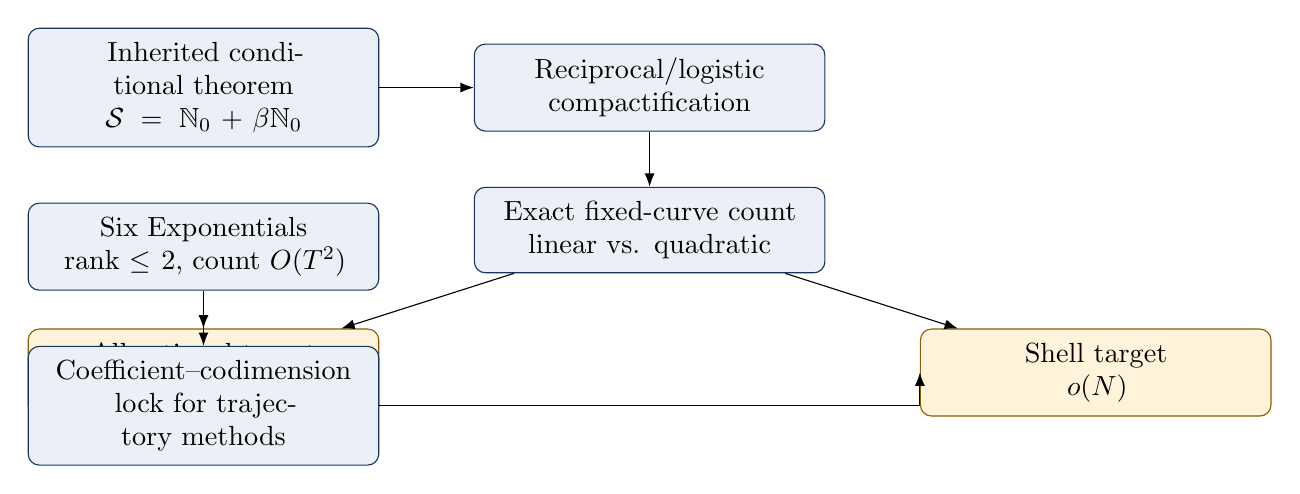
\begin{tikzpicture}[node distance=7mm and 12mm,>=Latex,
 box/.style={draw=navy,rounded corners,align=center,fill=bluegray,inner sep=5pt,text width=4.1cm},
 tbox/.style={draw=amber,rounded corners,align=center,fill=paleamber,inner sep=5pt,text width=4.1cm}]
\node[box] (inherited) {Inherited conditional theorem\\$\Sol=\Nzero+\beta\Nzero$};
\node[box,right=of inherited] (compact) {Reciprocal/logistic\\compactification};
\node[box,below=of compact] (count) {Exact fixed-curve count\\linear vs. quadratic};
\node[tbox,below left=of count] (allrat) {All-rational target\\$o(T^2)$};
\node[tbox,below right=of count] (shell) {Shell target\\$o(N)$};
\node[box,below=of inherited] (rank) {Six Exponentials\\rank $\le2$, count $O(T^2)$};
\node[box,below=of rank] (lock) {Coefficient--codimension\\lock for trajectory methods};
\draw[->] (inherited)--(compact);
\draw[->] (compact)--(count);
\draw[->] (count)--(allrat);
\draw[->] (count)--(shell);
\draw[->] (rank)--(allrat);
\draw[->] (rank)--(lock);
\draw[->] (lock.east) -| (shell.west);
\end{tikzpicture}
\end{center}

\section{Public-source audit and research boundary}

\subsection{The recent AI-mathematics claims}
Anthropic publicly announced Claude Fable 5 on 9 June 2026 and recorded its redeployment on 1 July 2026 \cite{AnthropicFable2026}.  The public record available during this investigation supports the following narrower formulations of the examples in the prompt.

\begin{itemize}
\item The Jacobian conjecture was publicly reported refuted in dimension three and then in every dimension greater than two; the cited preprint gives exact rational-arithmetic verification of explicit maps \cite{Gao2026}.  This is not a resolution of the still-distinct two-dimensional case.
\item Epoch AI reports a human--Claude team construction covering all previously unknown admissible Hadamard orders below 2000, including order 668, while explicitly noting that the general Hadamard conjecture remains open \cite{EpochHadamard2026}.
\item A public rank record gives an elliptic curve with thirty exhibited independent rational points, hence unconditional rank at least thirty; exact rank thirty is stated only under additional analytic conjectures in the source consulted \cite{MathWorldRank2026}.
\end{itemize}

These achievements justify taking the competitive claim seriously, but they do not supply mathematical evidence for a private Alaoglu--Erd\H{o}s argument.  A targeted search of official announcements, arXiv, public repositories, and mathematical discussion available on 23 August 2026 located no public preprint or formalization revealing such a method.  This is an audit statement about the search performed, not a claim that no private result exists.

\subsection{Truth boundary for this report}
\begin{cautionbox}
No inference in the mathematical body below relies on the existence or nonexistence of a rival proof.  The report uses only the supplied unified report, standard named theorems, the 2026 algebraic-relations paper, and arguments written out here.  Competitive framing is motivational; it is not evidence.
\end{cautionbox}

\subsection{Why the August 2026 relation-counting paper matters}
Binyamini, Hirata-Kohno, Kawashima, and Salant formulate a higher-codimension extension of Wilkie-type counting and prove a weaker small-ball covering theorem for compact pieces of polynomial differential trajectories satisfying an arithmetic \(D\)-property, in the range
\[
 k<\sqrt n-1
\]
for \(k\)-dimensional algebraic relations in ambient dimension \(n\) \cite{BHKKS2026}.  Their paper also explains that the full conjecture would imply open algebraic-independence results for multiplicative groups.  This makes it unusually relevant to the present problem.  The detailed audit in \cref{sec:relation-counting} shows both the opportunity and the exact mismatch.

\section{Foundational normalization and inherited structural input}
\label{sec:foundations}

\subsection{The exponent and the solution set}
Set
\[
 \thetaq:=\frac{\log 3}{\log 2}.
\]
For \(t\in\R\), the identity \(3^t=(2^t)^{\thetaq}\) identifies the original problem with integer points on the power curve \(y=x^{\thetaq}\).  Define
\[
 \Sol:=\{t\in\R:2^t\in\N,\ 3^t\in\N\}.
\]

\begin{lemma}[Elementary normalization; \statusP]
\label{lem:basic-theta}
The following statements hold.
\begin{enumerate}[label=\textup{(\roman*)}]
\item Every \(t\in\Sol\) is nonnegative.
\item \(\thetaq\) is irrational.
\item \(\thetaq\) is transcendental.
\item If \(q\in\Q\) and \(2^q\in\Q\), then \(q\in\Z\).  The same statement holds with base \(3\).
\end{enumerate}
\end{lemma}

\begin{proof}
If \(t<0\), then \(0<2^t<1\), so \(2^t\) cannot be a positive integer.  If \(\thetaq=a/b\in\Q\) in lowest terms, then \(2^a=3^b\), contradicting unique factorization.  If \(\thetaq\) were algebraic irrational, the Gelfond--Schneider theorem would make \(2^{\thetaq}\) transcendental, while \(2^{\thetaq}=3\).  Finally, if \(q=a/b\) in lowest terms and \(2^{a/b}=r/s\in\Q_{>0}\) in lowest terms, then \(2^a s^b=r^b\); prime valuations force \(b=1\).
\end{proof}

\subsection{The one inherited theorem used throughout}
The supplied report proves and formally verifies a much stronger conditional classification than is needed merely to state the conjecture.  We isolate it as an input rather than reproduce its long derivation.

\begin{theorem}[Canonical conditional monoid; \statusI]
\label{thm:inherited-monoid}
If the Alaoglu--Erd\H{o}s conjecture is false, there is a unique least nonintegral solution \(\beta>1\), necessarily irrational and transcendental, such that
\[
 \Sol=\{n+k\beta:n,k\in\Nzero\}.
\]
Writing
\[
 M:=2^\beta\in\N,\qquad A:=3^\beta\in\N,
\]
every solution and output pair have unique coordinates
\[
 t=n+k\beta,
 \qquad
 (2^t,3^t)=(2^nM^k,3^nA^k).
\]
In particular,
\begin{align}
 \#(\Sol\cap[N,N+1))
   &=1+\left\lfloor\frac{N+1}{\beta}\right\rfloor,\label{eq:inherited-shell}\\
 \#\{t\in\Sol:t\le X\}
   &=\frac{X^2}{2\beta}+O_\beta(X).\label{eq:inherited-cumulative}
\end{align}
\end{theorem}

\begin{remark}
The new constructions below use \cref{thm:inherited-monoid} only as a structural input.  Their compactification, exact height transfer, cusp geometry, rational dynamics, and differential obstruction are independent deductions.  In particular, the new fixed-compact count is not obtained by merely renaming the earlier modulo-one arc: the present maps are injective on the entire half-line and retain the integer-shift coordinate.
\end{remark}

\subsection{Two notions of rational height}
For a reduced rational number \(a/b\) with \(b>0\), put
\[
 H(a/b):=\max\{|a|,b\},\qquad h(a/b):=\log H(a/b).
\]
For \(P=(x_1,\ldots,x_r)\in\Q^r\), use the coordinate height
\[
 H(P):=\max_i H(x_i),\qquad h(P):=\log H(P).
\]
This is the height convention used in rational-point counting on affine sets.  It differs from the projective height of \([1:x_1:\cdots:x_r]\), but only by dimension-dependent powers; all logarithmic exponents discussed here are invariant under that change.  Exact formulas below refer to the coordinate height.

\section{The reciprocal compactification}
\label{sec:reciprocal}

\subsection{A fixed compact cusp with unit numerators}
Define the reciprocal power cusp
\[
 \rec:=\{(u,v)\in(0,1]^2:v=u^{\thetaq}\},
 \qquad
 \overline{\rec}:=\rec\cup\{(0,0)\}.
\]
The closure \(\overline{\rec}\subset[0,1]^2\) is compact.  Define
\[
 R:[0,\infty)\longrightarrow\rec,
 \qquad
 R(t):=(2^{-t},3^{-t}),
\]
and the unit-numerator set
\[
 \unitrec:=\left\{\left(\frac1m,\frac1n\right):m,n\in\N\right\}.
\]

\begin{theorem}[Reciprocal equivalence; \statusP]
\label{thm:reciprocal-equivalence}
The map \(R\) is injective, and for every \(t\ge0\),
\[
 t\in\Sol
 \quad\Longleftrightarrow\quad
 R(t)\in\unitrec.
\]
If \(t\in\Sol\), then
\[
 H(R(t))=3^t,
 \qquad
 h(R(t))=t\log3.
\]
\end{theorem}

\begin{proof}
Injectivity follows from injectivity of \(t\mapsto2^{-t}\).  If \(t\in\Sol\), write \(m=2^t\), \(n=3^t\); then \(R(t)=(1/m,1/n)\).  Conversely, if \(R(t)=(1/m,1/n)\), then \(2^t=m\) and \(3^t=n\) are positive integers.  For a marked point the two coordinates are reduced and have heights \(2^t\) and \(3^t\); since \(t\ge0\), the maximum is \(3^t\).
\end{proof}

\begin{provedbox}
The original unbounded integer-point problem has become a marked rational-point problem on one fixed compact curve.  No quotient by integer translation has occurred.  Every pair \((n,k)\) from a hypothetical rank-two solution monoid survives as a different point approaching the single cusp \((0,0)\).
\end{provedbox}

\subsection{Why this is not the one-point compactification}
A naive topological one-point compactification records that the orbit tends to infinity but destroys the relative rate of the two coordinates.  The reciprocal map is algebraic on the torus:
\[
 (x,y)\longmapsto(x^{-1},y^{-1}),
\]
and therefore preserves the full power relation, rationality, and logarithmic height.  The endpoint is not featureless: it is an irrational-exponent cusp whose exact regularity carries the arithmetic difficulty.

\subsection{A rank-preserving Möbius family}
The reciprocal chart is one member of a useful family.  For fixed \(c\in\Q_{>0}\), define
\[
 \psi_c(z):=\frac{z}{c+z}.
\]
This is a birational map of \(\Gm\) onto its image, with inverse \(z=cX/(1-X)\).

\begin{lemma}[Height stability under fixed Möbius compactification; \statusP]
\label{lem:mobius-height}
For fixed \(c\in\Q_{>0}\), there is a constant \(C_c\) such that for every \(z\in\Q_{>0}\),
\[
 |h(\psi_c(z))-h(z)|\le C_c.
\]
For every positive integer \(m\),
\[
 h\!\left(\frac{m}{m+1}\right)=\log(m+1).
\]
\end{lemma}

\begin{proof}
Write \(c=r/s\) in lowest terms and \(z=a/b\) in lowest terms.  Then
\[
 \psi_c(z)=\frac{as}{as+br}.
\]
After reduction, its numerator and denominator are bounded above by a fixed multiple of \(H(z)\).  Conversely, \(z=cX/(1-X)\) gives the reverse bound.  Taking logarithms proves the first assertion.  The second follows from \(\gcd(m,m+1)=1\).
\end{proof}

\begin{remark}
The choice \(c=1\) is arithmetically canonical: it produces reduced fractions whose denominator exceeds the numerator by exactly one.  Reciprocal inversion produces numerator one.  These are the two simplest rigid boundary conditions on rational points.
\end{remark}

\subsection{Visual geometry of the reciprocal chart}
\begin{center}
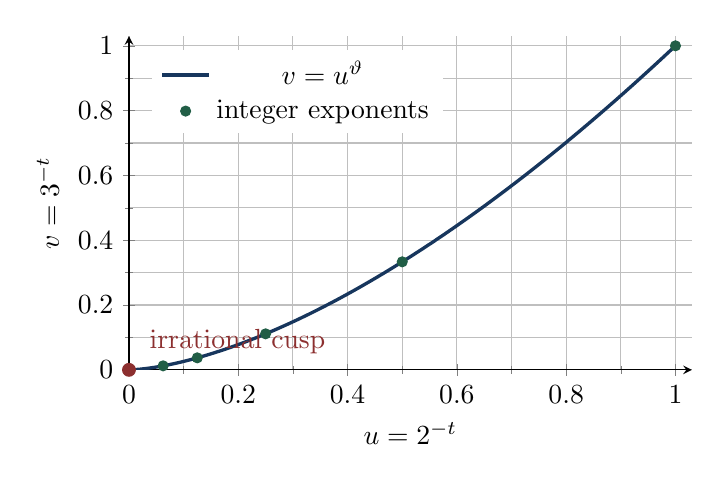
\begin{tikzpicture}
\begin{axis}[
 width=0.72\textwidth,height=0.48\textwidth,
 xmin=0,xmax=1.03,ymin=0,ymax=1.03,
 xlabel={$u=2^{-t}$},ylabel={$v=3^{-t}$},
 axis lines=left,grid=both,minor tick num=1,
 legend style={at={(0.04,0.96)},anchor=north west,fill=white,draw=none},
 samples=250]
\addplot[very thick,navy,domain=0.001:1] {x^(ln(3)/ln(2))};
\addlegendentry{$v=u^{\vartheta}$}
\addplot[only marks,mark=*,mark size=1.8pt,deepgreen]
 coordinates {(1,1) (0.5,0.3333333333) (0.25,0.1111111111) (0.125,0.0370370370) (0.0625,0.0123456790)};
\addlegendentry{integer exponents}
\addplot[only marks,mark=*,mark size=2.3pt,brick] coordinates {(0,0)};
\node[anchor=south west,text=brick] at (axis cs:0.02,0.02) {irrational cusp};
\end{axis}
\end{tikzpicture}
\end{center}

\section{The logistic/Farey compactification}
\label{sec:logistic}

\subsection{Conjugating the cusp to the Farey boundary}
Apply \(u\mapsto1/(1+u)\) in each reciprocal coordinate.  Equivalently define
\[
 \Phi(t):=\left(\frac{2^t}{1+2^t},\frac{3^t}{1+3^t}\right).
\]
For \(X\in(0,1)\), write
\[
 \logit(X):=\log\frac{X}{1-X}.
\]
The image curve is
\[
 \logcurve:=\left\{(X,Y)\in[1/2,1)^2:
 \logit(Y)=\thetaq\logit(X)\right\}.
\]
Solving for \(Y\) gives
\begin{equation}
 Y=F_{\thetaq}(X):=
 \frac{X^{\thetaq}}{X^{\thetaq}+(1-X)^{\thetaq}}.
 \label{eq:logistic-graph}
\end{equation}
Its closure adds the cusp \((1,1)\).

Define the coordinatewise unit-gap set
\[
 \unitgap:=\left\{\left(\frac{m}{m+1},\frac{n}{n+1}\right):m,n\in\N\right\}.
\]

\begin{theorem}[Unit-gap equivalence; \statusP]
\label{thm:unit-gap-equivalence}
The map \(\Phi:[0,\infty)\to\logcurve\) is injective, and
\[
 t\in\Sol
 \quad\Longleftrightarrow\quad
 \Phi(t)\in\unitgap.
\]
For \(t\in\Sol\),
\[
 H(\Phi(t))=3^t+1,
 \qquad
 h(\Phi(t))=\log(3^t+1)=t\log3+O(e^{-t\log3}).
\]
\end{theorem}

\begin{proof}
The first coordinate is strictly increasing in \(t\), so \(\Phi\) is injective.  The displayed unit-gap form is equivalent to \(2^t=m\) and \(3^t=n\).  Each fraction is reduced, and \(n\ge m\) for \(t\ge0\); hence the pair height is \(n+1=3^t+1\).
\end{proof}

\subsection{Farey-star interpretation}
Two reduced fractions \(a/b\) and \(c/d\) are adjacent in the Farey graph when \(|ad-bc|=1\).  For every \(m\ge1\),
\[
 \left|m\cdot1-(m+1)\cdot1\right|=1.
\]
Thus \(m/(m+1)\) is a Farey neighbor of the cusp \(1/1\).  Every marked point on \(\logcurve\) lies in the Cartesian product of the two Farey stars at \(1/1\).  This yields a compact arithmetic formulation with no reference to numerator prime support:
\[
 \boxed{
 \AEconj \iff
 \logcurve\cap\unitgap
 =\left\{\left(\frac{2^n}{2^n+1},\frac{3^n}{3^n+1}\right):n\in\Nzero\right\}.}
\]

\subsection{The two charts are rationally conjugate}
Let
\[
 \chi(u,v):=\left(\frac1{1+u},\frac1{1+v}\right).
\]
Then \(\Phi=\chi\circ R\), and \(\chi\) is birational with inverse
\[
 (X,Y)\longmapsto\left(\frac{1-X}{X},\frac{1-Y}{Y}\right).
\]

\begin{center}
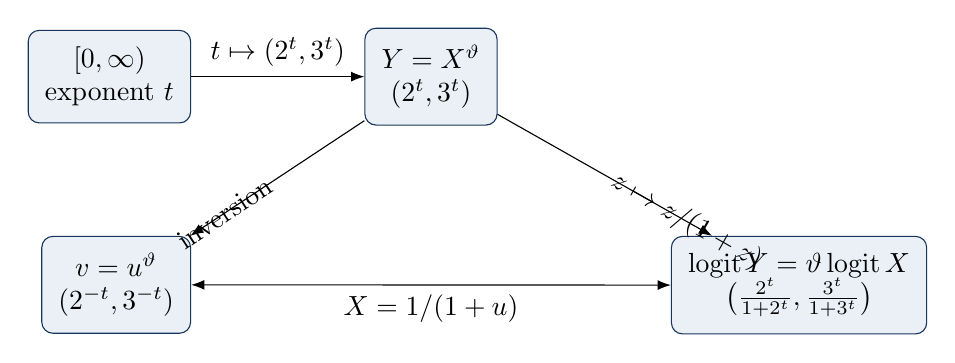
\begin{tikzpicture}[>=Latex,node distance=14mm and 22mm,
 every node/.style={align=center},
 map/.style={draw=navy,rounded corners,fill=bluegray,inner sep=6pt}]
\node[map] (line) {$[0,\infty)$\\exponent $t$};
\node[map,right=of line] (unbounded) {$Y=X^{\vartheta}$\\$(2^t,3^t)$};
\node[map,below left=of unbounded] (recip) {$v=u^{\vartheta}$\\$(2^{-t},3^{-t})$};
\node[map,below right=of unbounded] (logi) {$\logit Y=\vartheta\logit X$\\$\bigl(\frac{2^t}{1+2^t},\frac{3^t}{1+3^t}\bigr)$};
\draw[->] (line)--node[above] {$t\mapsto(2^t,3^t)$} (unbounded);
\draw[->] (unbounded)--node[left,sloped] {inversion} (recip);
\draw[->] (unbounded)--node[right,sloped] {$z\mapsto z/(1+z)$} (logi);
\draw[<->] (recip)--node[below] {$X=1/(1+u)$} (logi);
\end{tikzpicture}
\end{center}

\subsection{Why the logistic chart is useful}
The reciprocal chart has the cleanest exact height.  The logistic chart adds three complementary structures.
\begin{enumerate}
\item Every marked coordinate is represented by consecutive numerator and denominator.
\item The marked set is invariant under explicit rational self-maps of the interval, developed in \cref{sec:discrete-dynamics}.
\item The graph is strictly concave on \((1/2,1)\), so rational triples have a nonzero integer area numerator.  This creates a determinant certificate unavailable in the raw unbounded chart without first choosing a scale.
\end{enumerate}

\section{Exact counting on a fixed compact curve}
\label{sec:counting}

\subsection{The reciprocal marked count}
For \(T\ge0\), define
\[
 N_{\rm rec}(T):=
 \#\{P\in\rec\cap\unitrec:h(P)\le T\}.
\]
By \cref{thm:reciprocal-equivalence}, this is exactly
\[
 N_{\rm rec}(T)=
 \#\left\{t\in\Sol:t\le\frac{T}{\log3}\right\}.
\]
Likewise let
\[
 N_{\rm gap}(T):=
 \#\{P\in\logcurve\cap\unitgap:h(P)\le T\}.
\]

\begin{theorem}[Fixed-compact linear/quadratic dichotomy; \statusP+\statusI]
\label{thm:compact-dichotomy}
Exactly one of the following alternatives holds.
\begin{enumerate}[label=\textup{(\roman*)}]
\item If the Alaoglu--Erd\H{o}s conjecture is true, then
\[
 N_{\rm rec}(T)=\frac{T}{\log3}+O(1),
 \qquad
 N_{\rm gap}(T)=\frac{T}{\log3}+O(1).
\]
\item If the conjecture is false and \(\beta\) is the canonical generator from \cref{thm:inherited-monoid}, then
\begin{align*}
 N_{\rm rec}(T)
 &=\frac{T^2}{2\beta(\log3)^2}+O_\beta(T),\\
 N_{\rm gap}(T)
 &=\frac{T^2}{2\beta(\log3)^2}+O_\beta(T).
\end{align*}
\end{enumerate}
Consequently,
\begin{align}
 \AEconj
 &\iff N_{\rm rec}(T)=O(T)
  \iff N_{\rm rec}(T)=o(T^2),\label{eq:rec-equivalence}\\
 \AEconj
 &\iff N_{\rm gap}(T)=O(T)
  \iff N_{\rm gap}(T)=o(T^2).\label{eq:gap-equivalence}
\end{align}
\end{theorem}

\begin{proof}
If the conjecture holds, \(\Sol=\Nzero\), so the reciprocal count is
\(
\lfloor T/\log3\rfloor+1.
\)
For the logistic height, \(h(\Phi(t))\le T\) is equivalent to
\[
 t\le \log_3(e^T-1)
 =\frac{T}{\log3}+O(e^{-T}),
\]
which changes the integer count by \(O(1)\).

Under failure, \cref{thm:inherited-monoid} gives
\[
 N_{\rm rec}(T)=
 \sum_{0\le k\le L/\beta}
 \bigl(\lfloor L-k\beta\rfloor+1\bigr),
 \qquad L:=\frac{T}{\log3}.
\]
Replacing each floor by its argument incurs \(O(L)\), while summing the arithmetic progression gives \(L^2/(2\beta)+O_\beta(L)\).  The logistic cutoff differs from \(L\) by \(O(e^{-T})\), again affecting at most \(O(1)\) boundary points.  The equivalences follow because the two alternatives have distinct polynomial orders.
\end{proof}

\begin{provedbox}
The curve is fixed and compact in both alternatives.  The conditional second generator manifests itself as an extra logarithm in the rational-point count: rank one gives \(T\), rank two gives \(T^2\).  This is the central new reduction.
\end{provedbox}

\subsection{All-rational sufficient criteria}
Let
\[
 N_{\rm all}^{-}(T):=
 \#\{P\in\rec(\Q):h(P)\le T\},
\qquad
 N_{\rm all}^{+}(T):=
 \#\{P\in\logcurve(\Q):h(P)\le T\}.
\]
Since the marked sets are subsets of the full rational loci, \cref{thm:compact-dichotomy} gives immediately:

\begin{corollary}[All-rational fixed-curve criterion; \statusP]
\label{cor:all-rational-criterion}
Either of the bounds
\[
 N_{\rm all}^{-}(T)=o(T^2),
 \qquad
 N_{\rm all}^{+}(T)=o(T^2)
\]
would prove the Alaoglu--Erd\H{o}s conjecture.
\end{corollary}

\begin{remark}[Strength and price]
This criterion is stronger than the conjecture because it controls rational points not satisfying the unit-numerator or unit-gap condition.  Its advantage over the earlier compact fundamental arc is quantitative: a subquadratic exponent is enough, whereas quotienting by integer shifts leaves only a linear counterexample signal and therefore asks for a sublinear exponent.
\end{remark}

\subsection{Exact shell occupancy}
Define the reciprocal cusp shell
\[
 \mathscr S_N^-:=
 \left\{(u,v)\in\rec\cap\unitrec:
 2^{-N-1}<u\le2^{-N}\right\}.
\]
Since \(u=2^{-t}\), this is the image of \(\Sol\cap[N,N+1)\).

\begin{theorem}[Unit-shell census; \statusP+\statusI]
\label{thm:shell-census}
For every \(N\in\Nzero\):
\begin{enumerate}[label=\textup{(\roman*)}]
\item under the conjecture, \(\#\mathscr S_N^-=1\);
\item under failure,
\[
 \#\mathscr S_N^-
 =1+\left\lfloor\frac{N+1}{\beta}\right\rfloor
 =\frac{N}{\beta}+O_\beta(1).
\]
\end{enumerate}
Hence the conjecture is equivalent to bounded marked shell occupancy, and any estimate
\[
 \#\mathscr S_N^-=o(N)
\]
would prove it.
\end{theorem}

\begin{proof}
The shell condition is equivalent to \(N\le t<N+1\), and the count is \eqref{eq:inherited-shell}.  Under the conjecture the unique exponent in this interval is \(N\).
\end{proof}

\subsection{Renormalization explains the relation to the old compact arc}
For \(P=R(t)\in\mathscr S_N^-\), write \(t=N+s\) with \(0\le s<1\).  Multiplying by \((2^N,3^N)\) gives
\[
 (2^Nu,3^Nv)=(2^{-s},3^{-s}),
\]
a point on the fixed fundamental arc
\[
 \mathcal F^-:=\{(2^{-s},3^{-s}):0\le s<1\}.
\]
Under failure, the shell points are
\[
 t=N+\{k\beta\},
 \qquad
 0\le k\le\left\lfloor\frac{N+1}{\beta}\right\rfloor,
\]
with the convention \(k=0\) giving \(t=N\).  Thus shell renormalization recovers the synchronized rotation orbit studied in the supplied report.

The distinction is now transparent:
\begin{itemize}
\item the fundamental arc keeps the phase \(\{k\beta\}\) and discards the shell index \(N\), so its counterexample count is linear;
\item the compact cusp keeps both \(N\) and the phase, so summing the linearly growing shell occupancies produces a quadratic total.
\end{itemize}

\subsection{A synthetic lattice check}
The following table uses \(\beta=\sqrt2\) only to test the geometry of the formulas.  It is not an arithmetic candidate, since \(2^{\sqrt2}\) and \(3^{\sqrt2}\) are not asserted to be integers.

\begin{center}
\begin{tabular}{rrrrr}
\toprule
\(X\) & exact \(\#\{n+k\sqrt2\le X\}\) & \(X^2/(2\sqrt2)\) & error & exact/\(X^2\) \\
\midrule
10  & 45    & 35.355 & 9.645  & 0.4500 \\
20  & 160   & 141.421& 18.579 & 0.4000 \\
40  & 601   & 565.685& 35.315 & 0.3756 \\
80  & 2332  & 2262.742&69.258 & 0.3644 \\
160 & 9189  & 9050.967&138.033& 0.3589 \\
320 & 36478 & 36203.867&274.133&0.3562 \\
\bottomrule
\end{tabular}
\end{center}
The limiting normalized constant is \(1/(2\sqrt2)\approx0.353553\), while the error is linear, exactly as the lattice-area proof predicts.

\subsection{A hierarchy of sufficient bounds}
The compactification produces several logically distinct goals.
\begin{center}
\begin{tabularx}{0.97\textwidth}{p{0.27\textwidth}p{0.28\textwidth}X}
\toprule
Counting set & Sufficient bound & Comment \\
\midrule
Marked points on full compact cusp & \(o(T^2)\) & Exact equivalent; weakest arithmetic target in exponent. \\
All rational points on full cusp & \(o(T^2)\) & Stronger statement, no support restriction. \\
Marked points in shell \(N\) & \(o(N)\) & Exact local equivalent after summation. \\
All rational points in shell \(N\) & \(o(N)\) & Stronger local statement. \\
Marked points on normalized arc & \(o(T)\) & Earlier target; one logarithm harder. \\
All rational points on normalized arc & \(o(T)\) & Strongest generic fixed-arc target. \\
\bottomrule
\end{tabularx}
\end{center}

\section{The full rational-point group and the exact exponent-two ceiling}
\label{sec:rational-group}

\subsection{A multiplicative group on the power curve}
Define
\[
 \Gamma_{\thetaq}:=
 \{(r,s)\in\Q_{>0}^2:s=r^{\thetaq}\}.
\]
It is a subgroup of \(\Q_{>0}^2\) under coordinatewise multiplication.  Equivalently, let
\[
 G_{\thetaq}:=
 \{t\in\R:2^t,3^t\in\Q_{>0}\};
\]
then \(t\mapsto(2^t,3^t)\) is an isomorphism from the additive group \(G_{\thetaq}\) to \(\Gamma_{\thetaq}\).

\begin{theorem}[Six Exponentials rank ceiling; \statusE+\statusP]
\label{thm:six-exp-rank}
The group \(\Gamma_{\thetaq}\) is free abelian of rank at most two.
\end{theorem}

\begin{proof}
The group \(\Q_{>0}^2\) is a free abelian group under the two coordinatewise prime-valuation maps, so every subgroup is free abelian.  Suppose \(\Gamma_{\thetaq}\) had rank at least three.  Choose multiplicatively independent points corresponding to exponents \(t_1,t_2,t_3\in G_{\thetaq}\).  Multiplicative independence of the points is equivalent to \(\Q\)-linear independence of the \(t_i\).  The numbers \(\log2\) and \(\log3\) are also \(\Q\)-linearly independent.  The Six Exponentials Theorem \cite{Lang1966} then says that at least one of
\[
 e^{t_i\log2}=2^{t_i},
 \qquad
 e^{t_i\log3}=3^{t_i}
 \quad (i=1,2,3)
\]
is transcendental.  All six are rational by construction, a contradiction.
\end{proof}

\begin{remark}
This theorem is an upper bound of exactly the wrong sharpness for the conjecture.  A counterexample supplies the independent points \((2,3)\) and \((M,A)\), so rank two is genuinely compatible with every known unconditional transcendence theorem used here.  Four Exponentials would force rank one, but that is precisely the inaccessible barrier.
\end{remark}

\subsection{Height is a norm on a finitely generated rational group}
For \(P=(r,s)\in\Q_{>0}^2\), let \(h(P)=\log\max(H(r),H(s))\).

\begin{lemma}[Height-norm comparison; \statusP]
\label{lem:height-norm}
Let \(\Gamma\subset\Q_{>0}^2\) be a free abelian group of rank \(r<\infty\), with basis \(P_1,\ldots,P_r\).  There are constants \(0<c_\Gamma\le C_\Gamma\) such that for every \(\bm n=(n_1,\ldots,n_r)\in\Z^r\),
\[
 c_\Gamma\|\bm n\|_\infty
 \le h(P_1^{n_1}\cdots P_r^{n_r})
 \le C_\Gamma\|\bm n\|_\infty.
\]
\end{lemma}

\begin{proof}
Only finitely many primes occur in the basis coordinates.  Collecting their two coordinate valuation vectors gives an injective linear map
\[
 A:\R^r\longrightarrow\R^d
\]
for some finite \(d\).  Injectivity follows from multiplicative independence.  All norms on the finite-dimensional image are equivalent, so \(\|A\bm n\|\asymp\|\bm n\|\).  For a positive rational \(q=\prod p^{e_p}\),
\[
 \frac12\sum_p|e_p|\log p
 \le\log H(q)\le
 \sum_p|e_p|\log p.
\]
Applying this to both coordinates proves the comparison.
\end{proof}

\begin{corollary}[Unconditional quadratic ceiling; \statusE+\statusP]
\label{cor:quadratic-ceiling}
For either compact chart,
\[
 N_{\rm all}^{\pm}(T)=O_{\thetaq}(T^2).
\]
More precisely, if \(\rank\Gamma_{\thetaq}=r\), then the full rational-point count on any fixed compact branch meeting a positive cone in the exponent group is \(O(T^r)\).
\end{corollary}

\begin{proof}
Use \cref{thm:six-exp-rank,lem:height-norm}.  Points of height at most \(T\) correspond to lattice vectors in a box of side \(O(T)\), so there are \(O(T^r)\) of them.  Rational Möbius conjugacy changes height by \(O(1)\).
\end{proof}

\subsection{Rank two forces quadratic growth}
The upper bound is exact whenever the rational group has rank two.

\begin{proposition}[Rank/count equivalence; \statusP]
\label{prop:rank-count}
Let \(N_{\Gamma}^{-}(T)\) count all rational points of \(\rec\) of height at most \(T\).  Then
\[
 N_{\Gamma}^{-}(T)=o(T^2)
 \quad\Longleftrightarrow\quad
 \rank\Gamma_{\thetaq}=1.
\]
If the rank is two, then \(N_{\Gamma}^{-}(T)\asymp T^2\).
\end{proposition}

\begin{proof}
The rank-one case gives \(O(T)\) by \cref{lem:height-norm}.  In rank two, choose a basis and identify the logarithmic height with a norm on \(\R^2\).  The condition that the reciprocal point lie in \((0,1]^2\) is the half-space \(t\ge0\), where \(t\) is a nonzero real linear functional of the lattice coordinates.  A norm ball of radius \(T\) intersected with a nondegenerate half-space has area comparable to \(T^2\), and standard lattice counting gives \(\asymp T^2\) lattice points.  The finitely many points on the boundary do not affect the order.
\end{proof}

\begin{corollary}[Specialized Four Exponentials target; \statusP]
\label{cor:special-four-exp}
The all-rational subquadratic criterion of \cref{cor:all-rational-criterion} is equivalent to the assertion that every rational point on \(y=x^{\thetaq}\) belongs to the cyclic group generated by \((2,3)\).  This is the special rank-one consequence predicted by Four Exponentials.
\end{corollary}

\begin{proof}
If the rational group has rank one, it contains \((2,3)\).  This element is primitive: if \((2,3)=P^d\) with \(P\in\Q_{>0}^2\) and \(d>1\), then \(2\) and \(3\) would both be rational \(d\)-th powers, impossible by valuations.  Hence \(\Gamma_{\thetaq}=\langle(2,3)\rangle\).  Apply \cref{prop:rank-count}.
\end{proof}

\subsection{The integral cone inside a possible rank-two group}
The preceding all-rational criterion is stronger than Alaoglu--Erd\H{o}s.  The exact difference is polyhedral.

Assume for this subsection that \(\Gamma_{\thetaq}\) has rank two.  Because \((2,3)\) is primitive, choose a basis \(P_1=(2,3)\), \(P_2=(r,s)\).  Write a general group point as
\[
 P(n,k)=P_1^nP_2^k=(2^nr^k,3^ns^k),
 \qquad(n,k)\in\Z^2.
\]
For each prime \(p\), integrality imposes the two linear inequalities
\[
 n\,v_p(2)+k\,v_p(r)\ge0,
 \qquad
 n\,v_p(3)+k\,v_p(s)\ge0.
\]
Only finitely many are nontrivial.  Let \(\mathscr K\subset\R^2\) be their intersection.

\begin{theorem}[Valuation-cone reformulation; \statusP]
\label{thm:valuation-cone}
The set of integral rational points on the power curve is in bijection with
\[
 \mathscr K\cap\Z^2.
\]
The cone \(\mathscr K\) is a rational polyhedral cone containing the ray \(\R_{\ge0}(1,0)\).  Moreover,
\[
 \AEconj
 \quad\Longleftrightarrow\quad
 \mathscr K=\R_{\ge0}(1,0).
\]
If \(\mathscr K\) is larger than this ray, it contains an integral point with \(k\ne0\), hence a nonintegral solution after choosing the nonnegative exponent orientation.
\end{theorem}

\begin{proof}
The valuation inequalities are exactly the condition that both rational coordinates have no negative prime valuations.  Their coefficients are integers, so \(\mathscr K\) is rational polyhedral.  The allowed integer powers correspond to \((n,0)\), \(n\ge0\).  If the cone is larger, it contains either a second rational ray or a two-dimensional rational sector; in either case it contains a lattice point not on the first ray.  Its group point is integral and not a power of \((2,3)\), so its exponent is nonintegral by \cref{lem:basic-theta}.  The converse is immediate.
\end{proof}

\begin{remark}[New geometric meaning of the conjecture]
Six Exponentials reduces the global rational geometry to rank at most two.  Within the remaining rank-two possibility, Alaoglu--Erd\H{o}s says that the positive valuation cone degenerates to one boundary ray.  A counterexample opens that cone to dimension two, and quadratic counting is simply the Ehrhart-type growth of lattice points in the opened cone.
\end{remark}

\section{Cusp geometry, concavity, and integer area certificates}
\label{sec:cusp-geometry}

\subsection{Regularity of the reciprocal cusp}
Let \(f(u)=u^{\thetaq}\) on \([0,1]\), with \(f(0)=0\).  Since \(1<\thetaq<2\),
\[
 f'(u)=\thetaq u^{\thetaq-1},
 \qquad
 f''(u)=\thetaq(\thetaq-1)u^{\thetaq-2}.
\]

\begin{proposition}[Exact endpoint regularity; \statusP]
\label{prop:cusp-regularity}
The compact reciprocal graph is \(C^1\) at \((0,0)\), with horizontal tangent, but it is not \(C^2\) there.  It is strictly convex on \((0,1]\), and
\[
 f''(u)\longrightarrow+\infty
 \qquad(u\downarrow0).
\]
\end{proposition}

\begin{proof}
Because \(\thetaq>1\), \(f'(u)\to0\).  Because \(\thetaq<2\), the exponent \(\thetaq-2\) is negative, so \(f''\to+\infty\).  Positivity of \(f''\) gives strict convexity.
\end{proof}

\begin{remark}
All rational-point growth is concentrated at the unique boundary singularity.  Every closed subarc \(u\in[\varepsilon,1]\) is real analytic and of bounded Pfaffian complexity.  A global argument must therefore be scaling-covariant: treating increasingly small cusp shells as unrelated analytic arcs pays an avoidable logarithmic cost.
\end{remark}

\subsection{Differential geometry of the logistic curve}
Write \(F=F_{\thetaq}\) as in \eqref{eq:logistic-graph}.  Differentiating \(\logit F=\thetaq\logit X\) gives
\begin{align}
 F'(X)
 &=\thetaq\frac{F(X)(1-F(X))}{X(1-X)},\label{eq:Fprime}\\
 F''(X)
 &=\thetaq\frac{F(X)(1-F(X))}{X^2(1-X)^2}
 \left[\thetaq(1-2F(X))-(1-2X)\right].\label{eq:Fsecond}
\end{align}

\begin{proposition}[Strict concavity and cusp asymptotics; \statusP]
\label{prop:logistic-concavity}
For \(1/2<X<1\), one has \(F(X)>X\) and \(F''(X)<0\).  If \(s=1-X\downarrow0\), then
\begin{align}
 1-F(1-s)&=s^{\thetaq}(1+O(s)),\label{eq:logistic-cusp}\\
 F''(1-s)&=-\thetaq(\thetaq-1)s^{\thetaq-2}(1+o(1)).\label{eq:logistic-curvature}
\end{align}
Thus the logistic closure is also \(C^1\) but not \(C^2\) at its cusp \((1,1)\).
\end{proposition}

\begin{proof}
For \(X>1/2\), \(\logit X>0\), so multiplication by \(\thetaq>1\) gives \(F(X)>X\).  In the bracket of \eqref{eq:Fsecond}, set \(a=2F-1\) and \(b=2X-1\).  Then \(a>b>0\), so
\[
 \thetaq(1-2F)-(1-2X)=-\thetaq a+b<-a+b<0.
\]
This proves strict concavity.  Also
\[
 1-F(1-s)
 =\frac{s^{\thetaq}}{s^{\thetaq}+(1-s)^{\thetaq}}
 =s^{\thetaq}(1+O(s)).
\]
Differentiating the leading regular-variation term, or substituting it into \eqref{eq:Fsecond}, yields \eqref{eq:logistic-curvature}.
\end{proof}

\begin{center}
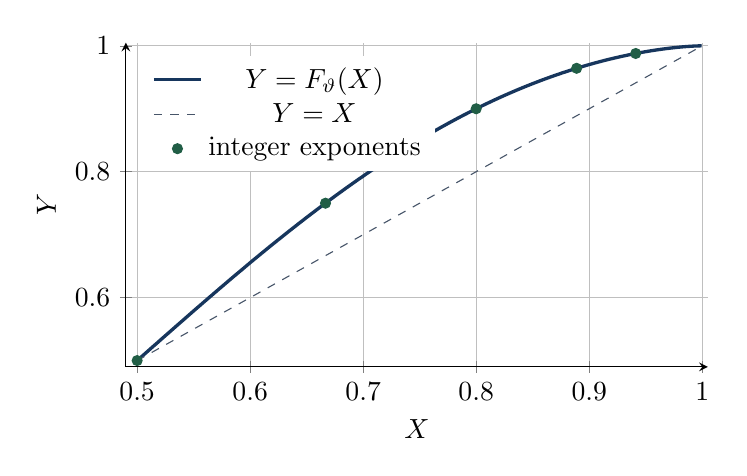
\begin{tikzpicture}
\begin{axis}[
 width=0.74\textwidth,height=0.47\textwidth,
 xmin=0.49,xmax=1.005,ymin=0.49,ymax=1.005,
 xlabel={$X$},ylabel={$Y$},axis lines=left,grid=both,
 legend style={at={(0.03,0.96)},anchor=north west,fill=white,draw=none},
 samples=250]
\addplot[very thick,navy,domain=0.5:0.9995]
 {x^(ln(3)/ln(2))/(x^(ln(3)/ln(2))+(1-x)^(ln(3)/ln(2)))};
\addlegendentry{$Y=F_{\vartheta}(X)$}
\addplot[dashed,slate,domain=0.5:1] {x};
\addlegendentry{$Y=X$}
\addplot[only marks,mark=*,mark size=1.8pt,deepgreen]
 coordinates {(0.5,0.5) (0.6666666667,0.75) (0.8,0.9) (0.8888888889,0.9642857143) (0.9411764706,0.9878048780)};
\addlegendentry{integer exponents}
\end{axis}
\end{tikzpicture}
\end{center}

\subsection{An exact integer numerator for three marked points}
Let \(X_i=m_i/(m_i+1)\), \(Y_i=n_i/(n_i+1)\), where \(m_i,n_i\in\N\), and define the oriented area determinant
\[
 \Delta(P_1,P_2,P_3):=
 \det\begin{pmatrix}
 1&X_1&Y_1\\
 1&X_2&Y_2\\
 1&X_3&Y_3
 \end{pmatrix}.
\]

\begin{proposition}[Unit-gap determinant certificate; \statusP]
\label{prop:unit-gap-determinant}
Suppose \(P_i=(X_i,F(X_i))\in\logcurve\cap\unitgap\) and
\(X_1<X_2<X_3\).  Then \(\Delta<0\), and
\begin{equation}
 \Delta=
 \frac{D}{\prod_{i=1}^3(m_i+1)(n_i+1)},
 \qquad
 D=\det\begin{pmatrix}
 (m_1+1)(n_1+1)&n_1+1&m_1+1\\
 (m_2+1)(n_2+1)&n_2+1&m_2+1\\
 (m_3+1)(n_3+1)&n_3+1&m_3+1
 \end{pmatrix}
 \in\Z\setminus\{0\}.
\label{eq:integer-area}
\end{equation}
Consequently,
\begin{equation}
 |\Delta|\ge
 \frac1{\prod_{i=1}^3(m_i+1)(n_i+1)}.
\label{eq:area-lower}
\end{equation}
There is also \(\xi\in(X_1,X_3)\) such that
\begin{equation}
 \Delta=\frac{F''(\xi)}2
 \prod_{1\le i<j\le3}(X_j-X_i),
\label{eq:area-upper-exact}
\end{equation}
and
\begin{equation}
 X_j-X_i=\frac{m_j-m_i}{(m_i+1)(m_j+1)}.
\label{eq:unit-gap-difference}
\end{equation}
\end{proposition}

\begin{proof}
Strict concavity gives \(\Delta<0\).  Multiply row \(i\) by \((m_i+1)(n_i+1)\).  The resulting row is
\[
 ((m_i+1)(n_i+1),\ m_i(n_i+1),\ n_i(m_i+1)).
\]
Subtracting the first column from each of the last two and changing both signs yields the integer determinant in \eqref{eq:integer-area}.  It is nonzero because \(\Delta\ne0\), proving \eqref{eq:area-lower}.  Formula \eqref{eq:area-upper-exact} is the standard second divided-difference identity; \eqref{eq:unit-gap-difference} is direct subtraction.
\end{proof}

\begin{remark}[What the three-point certificate does and does not do]
The lower bound is arithmetic and exact; the upper bound is geometric and exact.  Their present exponents do not contradict one another.  Near the cusp, the divergence of \(|F''|\) compensates for part of the small horizontal spacing.  The certificate is therefore a local exclusion tool, not a proof.  Its value is that it is adapted to the unit-gap denominators and can be iterated in higher-order determinants without first undoing the compactification.
\end{remark}

\subsection{A shell separation lemma from logarithmic forms}
Assume failure and write the shell exponents as
\[
 t_k=N+\{k\beta\},
 \qquad
 0\le k\le\left\lfloor\frac{N+1}{\beta}\right\rfloor.
\]
Because \(M=2^\beta\) and \(2\) are multiplicatively independent algebraic numbers, a standard lower bound for a nonzero linear form in two logarithms \cite{BakerWustholz2007} gives constants \(c,C>0\), depending on the hypothetical \(M\), such that
\[
 \|q\beta\|_{\R/\Z}\ge c q^{-C}
 \qquad(q\ge1).
\]

\begin{proposition}[Polynomial shell separation; \statusE+\statusP]
\label{prop:shell-separation}
Under failure, distinct normalized shell points
\[
 (2^{-\{k\beta\}},3^{-\{k\beta\}})
\]
with \(k\ll N\) are separated in Euclidean distance by at least \(c'N^{-C'}\), for constants depending on \(M\).  In particular, for every fixed \(\rho>0\), balls of radius \(e^{-N^\rho}\) contain at most one such point for all sufficiently large \(N\).
\end{proposition}

\begin{proof}
The difference between two phases is \(\|(k-\ell)\beta\|\), which has the stated polynomial lower bound.  On the compact interval \([0,1]\), the parametrization \(s\mapsto(2^{-s},3^{-s})\) has derivative bounded above and bounded away from zero in norm.  Hence phase distance and Euclidean distance are comparable.  Finally, every polynomial reciprocal dominates \(e^{-N^\rho}\) as \(N\to\infty\).
\end{proof}

\begin{remark}
This observation converts a sufficiently strong small-ball covering theorem into a cardinality theorem on each shell.  The current trajectory theorem still has two independent deficits: it does not apply to the natural lift in the needed codimension, and its polynomial covering exponent is not known to be below one.  See \cref{sec:relation-counting}.
\end{remark}

\subsection{Ford-circle picture}
The Ford circle at a reduced fraction \(a/q\) has radius \(1/(2q^2)\).  A marked logistic coordinate \(m/(m+1)\) therefore corresponds to a circle tangent to the cusp circle at \(1/1\), with radius \(1/[2(m+1)^2]\).  Along a solution point,
\[
 n=3^t=(2^t)^{\thetaq}=m^{\thetaq},
\]
so the two Ford radii satisfy asymptotically
\[
 \rho_Y\asymp \rho_X^{\thetaq}.
\]
The conjecture can thus be viewed as a rigidity statement for pairs of Ford circles in two cusp stars linked by an irrational Hölder law.  This interpretation is not itself a proof, but it suggests importing hyperbolic cusp counting and Farey transfer operators into a setting where the arithmetic subset is geometrically canonical.

\section{What generic rational-point counting gives, and why it misses}
\label{sec:generic-counting}

\subsection{Pfaffian complexity}
On an interval avoiding the cusp, the logistic graph is Pfaffian.  One convenient chain is
\[
 g(X)=\frac1{X(1-X)},
 \qquad
 F(X),
\]
with differential equations
\[
 g'=-(1-2X)g^2,
 \qquad
 F'=\thetaq gF(1-F).
\]
Thus the natural chain order is \(r=2\).  The reciprocal graph \(u^{\thetaq}\) likewise has a chain of order two on \((0,1]\).

Pila's explicit 2007 theorem for a nonalgebraic Pfaffian graph of order \(r\) gives a bound
\[
 N(H)\ll(\log H)^{5(r+2)},
\]
so the off-the-shelf exponent here is twenty \cite{Pila2007}.  The 2024 theorem of Binyamini--Novikov--Zak proves a polylogarithmic bound for restricted sub-Pfaffian structures and, as a corollary, Wilkie's conjecture for \(\R_{\exp}\), but does not provide a universal exponent below two for this curve \cite{BNZ2024}.

\begin{cautionbox}
``Polylogarithmic'' is not enough.  A counterexample supplies \(\asymp(\log H)^2\) marked points on the compact cusp.  To contradict it, the exponent must be strictly less than two, or the estimate must use the unit-numerator/unit-gap arithmetic.  Bounds such as \((\log H)^{20}\) are qualitatively impressive and quantitatively inert here.
\end{cautionbox}

\subsection{Why the cusp is the entire issue}
For fixed \(\varepsilon>0\), the segment \(u\in[\varepsilon,1]\) has bounded height for unit-numerator points, because \(u=1/m\ge\varepsilon\) implies \(m\le1/\varepsilon\).  As \(H\to\infty\), every new marked point lies in the cusp region \(u\ll1\).  One may cover this region by dyadic shells, rescale each shell to the fundamental arc, and apply a uniform analytic estimate.  But summing shellwise bounds introduces an extra logarithm unless the argument couples the shells.  The desired method must exploit the exact scaling
\[
 (u,v)\mapsto(u/2,v/3)
\]
rather than regard each shell as unrelated.

\subsection{A scaling-covariant determinant target}
The standard determinant method selects monomials, evaluates them at rational points, obtains a denominator lower bound for a nonzero determinant, and compares it with an analytic upper bound.  On the cusp, the monomial \(u^iv^j\) has scaling weight
\[
 i+j\thetaq.
\]
Under \((u,v)\mapsto(u/2,v/3)\), it is multiplied by \(2^{-i}3^{-j}\).  This diagonal action suggests choosing interpolation spaces by weight rather than total degree and performing row operations simultaneously across shells.

\begin{problem}[Scaling-covariant determinant theorem; \statusT]
\label{prob:scaling-determinant}
Prove that the number of unit-numerator rational points on
\(v=u^{\thetaq}\) with \(h(u,v)\le T\) is
\[
 O(T^{2-\delta})
\]
for some \(\delta>0\), by a determinant whose monomial set is stable under the \((2,3)\)-scaling and whose denominator divisibility is accumulated across all shells before the archimedean estimate is applied.
\end{problem}

The key novelty required by \cref{prob:scaling-determinant} is not a larger determinant.  It is an extra source of size that survives the exact compensation between cusp curvature and rational denominators.  Candidate sources are:
\begin{enumerate}
\item common divisibility forced by the unit numerator in both coordinates;
\item cross-shell row operations using the rational map \((u,v)\mapsto(u/2,v/3)\);
\item a weighted Newton basis adapted to the ordered semigroup \(i+j\thetaq\);
\item an adelic estimate in which fresh primes of \(m+1\) and \(n+1\) contribute through the logistic chart.
\end{enumerate}


\subsection{Exponential alternants: an exact denominator ledger}
The reciprocal chart makes the usual interpolation determinant unusually transparent.  Put
\[
 a:=\log 2,\qquad b:=\log 3,
\]
and let
\(
 \Lambda=\{(p_j,q_j):1\le j\le D\}\subset\Nzero^2
\)
be a finite monomial set.  Its weights are
\[
 \lambda_j:=ap_j+bq_j.
\]
They are pairwise distinct because \(a/b\notin\Q\).  At parameters
\(t_1<\cdots<t_D\), the evaluation determinant is
\begin{equation}
 \mathscr A_\Lambda(\bm t)
 :=\det\!\left((2^{-t_i})^{p_j}(3^{-t_i})^{q_j}\right)_{i,j=1}^D
 =\det\!\left(e^{-\lambda_jt_i}\right)_{i,j=1}^D.
\label{eq:exponential-alternant}
\end{equation}

\begin{proposition}[Strict sign-regularity; \statusP]
\label{prop:alternant-sign}
Order the weights so that \(\lambda_1<\cdots<\lambda_D\).  Then
\[
 (-1)^{D(D-1)/2}\mathscr A_\Lambda(\bm t)>0
 \qquad(t_1<\cdots<t_D).
\]
In particular, no such monomial evaluation determinant vanishes at distinct points of the power curve.
\end{proposition}

\begin{proof}
The Wronskian of the functions \(e^{-\lambda_jt}\) is
\[
 \det\left((-\lambda_j)^{i-1}e^{-\lambda_jt}\right)_{i,j=1}^D
 =(-1)^{D(D-1)/2}e^{-t\sum_j\lambda_j}
   \prod_{1\le i<j\le D}(\lambda_j-\lambda_i),
\]
which never vanishes and has the displayed sign.  Every initial subsystem has the same property.  Hence the ordered exponentials form an extended complete Chebyshev system, and its evaluation alternants have the Wronskian sign.
\end{proof}

This nonvanishing is stronger than the generic determinant method needs: there is no exceptional algebraic subcurve on which the determinant can disappear.  It also gives an exact arithmetic lower bound.

\begin{proposition}[Unit-numerator lower bound; \statusP]
\label{prop:alternant-lower}
Suppose \(t_i\in\Sol\), and write \(m_i=2^{t_i}\), \(n_i=3^{t_i}\).  Put
\[
 P:=\max_jp_j,\qquad Q:=\max_jq_j,
 \qquad W_{\max}:=aP+bQ.
\]
Then
\begin{equation}
 |\mathscr A_\Lambda(\bm t)|
 \ge \prod_{i=1}^D m_i^{-P}n_i^{-Q}
 =\exp\!\left(-W_{\max}\sum_{i=1}^Dt_i\right).
\label{eq:alternant-lower}
\end{equation}
\end{proposition}

\begin{proof}
Multiply row \(i\) of the determinant by \(m_i^Pn_i^Q\).  Every resulting entry is the integer
\(m_i^{P-p_j}n_i^{Q-q_j}\).  By \cref{prop:alternant-sign}, the resulting integer determinant is nonzero, so its absolute value is at least one.  Dividing by the row factors gives \eqref{eq:alternant-lower}.
\end{proof}

There is also a clean archimedean upper bound.  Denote
\[
 V(\bm t):=\prod_{1\le i<j\le D}(t_j-t_i),
 \qquad
 V(\bm\lambda):=\prod_{1\le i<j\le D}(\lambda_j-\lambda_i).
\]

\begin{proposition}[HCIZ upper bound; \statusE+\statusP]
\label{prop:alternant-upper}
For \(t_1<\cdots<t_D\) and \(0\le\lambda_1<\cdots<\lambda_D\),
\begin{equation}
 |\mathscr A_\Lambda(\bm t)|
 \le
 e^{-t_1\sum_j\lambda_j}
 \frac{V(\bm t)V(\bm\lambda)}{\prod_{r=1}^{D-1}r!}.
\label{eq:alternant-upper}
\end{equation}
\end{proposition}

\begin{proof}
Factor \(e^{-t_1\lambda_j}\) from column \(j\), and put
\(s_i=t_i-t_1\).  The Harish--Chandra--Itzykson--Zuber formula \cite{HCIZ} expresses
\[
 \det(e^{-s_i\lambda_j})
 =\frac{V(-\bm s)V(\bm\lambda)}{\prod_{r=1}^{D-1}r!}
 \int_{U(D)}
   \exp\!\bigl(\operatorname{tr}(-S U\Lambda U^*)\bigr)\,dU,
\]
up to the sign already fixed in \cref{prop:alternant-sign}, where
\(S=\operatorname{diag}(s_i)\), \(\Lambda=\operatorname{diag}(\lambda_j)\), and Haar measure is normalized.  Both \(S\) and \(U\Lambda U^*\) are positive semidefinite, so the trace in the exponent is nonpositive and the integral is at most one.  Taking absolute values gives \eqref{eq:alternant-upper}.
\end{proof}

\subsection{The monomial denominator deficit}
Combining \cref{prop:alternant-lower,prop:alternant-upper} for points in one shell reveals a precise obstruction.  Define
\begin{equation}
 \mathfrak d(\Lambda)
 :=D(aP+bQ)-\sum_{(p,q)\in\Lambda}(ap+bq)
 =a\sum_{(p,q)\in\Lambda}(P-p)
  +b\sum_{(p,q)\in\Lambda}(Q-q).
\label{eq:deficit}
\end{equation}
It is the gap between the denominator weight paid row by row and the average analytic decay carried column by column.

\begin{proposition}[Shell ledger; \statusP]
\label{prop:shell-ledger}
If \(N\le t_1<\cdots<t_D<N+1\) are marked points, then
\begin{equation}
 1\le
 \exp\!\bigl(N\mathfrak d(\Lambda)+D(aP+bQ)\bigr)
 \frac{V(\bm t)V(\bm\lambda)}{\prod_{r=1}^{D-1}r!}.
\label{eq:shell-ledger}
\end{equation}
Consequently, an ordinary monomial determinant can contradict the existence of \(D\) points in the shell only if some additional arithmetic divisibility or analytic cancellation compensates the term \(N\mathfrak d(\Lambda)\).
\end{proposition}

\begin{proof}
In \eqref{eq:alternant-lower}, use
\(\sum_i t_i<D(N+1)\).  In \eqref{eq:alternant-upper}, use \(t_1\ge N\).  Dividing the upper bound by the lower bound gives \eqref{eq:shell-ledger}.
\end{proof}

The deficit is invariant under translating every exponent pair by the same lattice vector.  Allowing Laurent monomials therefore does not remove it.  More importantly, its optimal order can be computed exactly.

\begin{theorem}[Optimal monomial-deficit asymptotic; \statusP]
\label{thm:deficit-asymptotic}
Let
\[
 \delta_D:=\min\{\mathfrak d(\Lambda):
       \Lambda\subset\Nzero^2,\ |\Lambda|=D\}.
\]
Then
\begin{equation}
 \delta_D=\frac{2^{3/2}}{3}\sqrt{ab}\,D^{3/2}+O_{a,b}(D).
\label{eq:deficit-asymptotic}
\end{equation}
In particular, every plain two-variable monomial determinant has an unavoidable shell loss \(\gg ND^{3/2}\) in its logarithmic size ledger.
\end{theorem}

\begin{proof}
Reflect \(\Lambda\) in its north-east corner:
\[
 \Lambda^\vee:=\{(P-p,Q-q):(p,q)\in\Lambda\}.
\]
Then \(\mathfrak d(\Lambda)\) is the sum of the weights \(ai+bj\) over \(\Lambda^\vee\).  Conversely, after translating a finite subset of \(\Nzero^2\) down to the coordinate axes and reflecting it in a sufficiently large corner, one recovers a monomial set with the same weight sum.  Therefore \(\delta_D\) is the sum of the \(D\) smallest elements, counted with their lattice multiplicities, of
\[
 \{ai+bj:i,j\in\Nzero\}.
\]
The irrationality of \(a/b\) makes these weights distinct, although the asymptotic does not require this.

Let
\[
 A(R):=\#\{(i,j)\in\Nzero^2:ai+bj\le R\},
 \quad
 S(R):=\sum_{ai+bj\le R}(ai+bj).
\]
Elementary lattice-point summation in the triangle \(ax+by\le R\) gives
\[
 A(R)=\frac{R^2}{2ab}+O_{a,b}(R),
 \qquad
 S(R)=\frac{R^3}{3ab}+O_{a,b}(R^2).
\]
If \(R_D\) is the \(D\)-th smallest weight, then
\[
 R_D=\sqrt{2abD}+O_{a,b}(1).
\]
The discrepancy between \(D\) and \(A(R_D)\) changes the partial sum by only \(O(R_D^2)=O(D)\).  Hence
\[
 \delta_D
 =\frac{R_D^3}{3ab}+O(D)
 =\frac{2^{3/2}}3\sqrt{ab}\,D^{3/2}+O(D),
\]
as asserted.
\end{proof}

\begin{cautionbox}
The theorem is a negative result about a method, not about the conjecture.  Total positivity guarantees that the determinant is nonzero; the unit numerator gives the best immediate integer lower bound; but the north-east denominator deficit still grows as \(D^{3/2}\).  Increasing the determinant size without adding new divisibility makes the shell loss worse.  A successful determinant proof must change the arithmetic ledger, not merely optimize the monomial shape.
\end{cautionbox}

\subsection{What extra divisibility would suffice}
Suppose that, after the row denominators in \cref{prop:alternant-lower} are cleared, the resulting integer determinant is always divisible by an integer \(\mathfrak M\).  The lower bound improves by a factor \(\mathfrak M\), and \eqref{eq:shell-ledger} becomes
\[
 \mathfrak M\le
 \exp\!\bigl(N\mathfrak d(\Lambda)+D(aP+bQ)\bigr)
 \frac{V(\bm t)V(\bm\lambda)}{\prod_{r=1}^{D-1}r!}.
\]
Thus the natural quantitative target is
\begin{equation}
 \log\mathfrak M
 \ge (1+\varepsilon)N\mathfrak d(\Lambda)
      +\text{the explicit Vandermonde error}
\label{eq:needed-divisibility}
\end{equation}
for a sequence of shell-adapted monomial sets.  The factor \(N\) shows why pointwise denominator estimates are unlikely to suffice: the divisibility must accumulate under repeated use of the exact contraction \((u,v)\mapsto(u/2,v/3)\).

Two concrete devices deserve testing.

\paragraph{Scaling differences.}
For a polynomial \(P(u,v)\), define
\[
 \Delta_{2,3}P(u,v):=P(u,v)-P(u/2,v/3).
\]
On a marked orbit this compares adjacent integer shifts.  On monomials it acts diagonally:
\[
 \Delta_{2,3}(u^pv^q)=(1-2^{-p}3^{-q})u^pv^q.
\]
After clearing powers of \(2\) and \(3\), iterated scaling differences produce factors \(2^p3^q-1\).  The open question is whether a multivariate Newton basis built from these operators forces enough common divisibility in the evaluation determinant to meet \eqref{eq:needed-divisibility}.

\paragraph{Unit-gap Newton factors.}
In the logistic chart, the cusp variables are
\[
 1-X=\frac1{m+1},\qquad 1-Y=\frac1{n+1}.
\]
Differences between rows carry exact integer numerators
\[
 X_j-X_i=\frac{m_j-m_i}{(m_i+1)(m_j+1)},
 \quad
 Y_j-Y_i=\frac{n_j-n_i}{(n_i+1)(n_j+1)}.
\]
A Newton determinant therefore sees the factors \(m_j-m_i\) and \(n_j-n_i\), which are absent from the crude row-denominator lower bound.  A counterexample would specialize these to differences in the two semigroups \(2^nM^k\) and \(3^nA^k\).  The required theorem is a simultaneous lower bound for the aggregate divisibility of these two difference products.

\begin{problem}[Simultaneous semigroup Vandermonde gain; \statusT]
\label{prob:semigroup-vandermonde}
Let \(M,A\ge2\) satisfy \(\log M/\log2=\log A/\log3\notin\Q\).  For lattice points \((n_i,k_i)\) in a unit exponent shell, quantify the product of nonarchimedean gains in
\[
 \prod_{i<j}(2^{n_j}M^{k_j}-2^{n_i}M^{k_i})
 \quad\text{and}\quad
 \prod_{i<j}(3^{n_j}A^{k_j}-3^{n_i}A^{k_i})
\]
relative to the archimedean size.  A gain of order \(\exp(cND^{3/2})\) in a suitable mixed determinant would overcome the optimal monomial deficit.
\end{problem}


\section{The 2026 algebraic-relation theorem: opportunity and exact lock}
\label{sec:relation-counting}

\subsection{The theorem in the form relevant here}
Binyamini, Hirata-Kohno, Kawashima, and Salant consider algebraic relations met by compact trajectories of polynomial vector fields over number fields.  In the notation needed here, their 2026 theorem says the following \cite{BHKKS2026}.

\begin{theorem}[Small-ball covering for algebraic relations; \statusE]
\label{thm:bhkks}
Let \(\Gamma\) be a compact analytic piece of a trajectory of a polynomial vector field on \(\C^n\), defined over a number field, and suppose the trajectory satisfies the arithmetic \(D\)-property.  For \(\rho\ge1\) and
\[
 k<\sqrt n-1,
\]
the points of \(\Gamma\) lying on algebraic varieties of dimension \(k\), degree at most \(g\), and logarithmic height at most \(h\), are covered by
\[
 (g+h)^{\rho C}
\]
balls of radius \(\exp(-(g+h)^\rho)\), where \(C\) depends on the trajectory, vector field, and number field.
\end{theorem}

The paper also formulates a stronger general relation-counting conjecture and explains that such results have consequences beyond the current state of algebraic independence for one-parameter multiplicative groups.  This is precisely the conceptual neighborhood of Alaoglu--Erd\H{o}s: the arithmetic event fixes two exponential coordinates while leaving a hidden transcendental parameter.

\subsection{Why the natural two-dimensional differential equation is illegal}
We begin with a small lemma that will be used repeatedly.

\begin{lemma}[Zariski density of the irrational power graph; \statusP]
\label{lem:zariski-power}
If \(\alpha\notin\Q\), then
\[
 \{(x,x^\alpha):x>0\}
\]
is Zariski dense in \(\A^2_\C\).  Its image under any birational automorphism of the two-dimensional torus is likewise Zariski dense.
\end{lemma}

\begin{proof}
If \(R(X,Y)=\sum c_{ij}X^iY^j\) vanishes on the graph, then
\[
 \sum c_{ij}x^{i+j\alpha}=0\qquad(x>0).
\]
The exponents \(i+j\alpha\) are pairwise distinct.  After setting \(x=e^s\), this is a finite linear combination of distinct real exponentials in \(s\), hence all coefficients vanish.  Birational maps preserve Zariski density on their domains.
\end{proof}

Recall that \(\thetaq\) is transcendental: it is irrational by unique factorization, and if it were algebraic irrational then Gelfond--Schneider would make \(2^{\thetaq}=3\) transcendental.

\begin{theorem}[Planar coefficient obstruction; \statusP]
\label{thm:planar-obstruction}
Let \(K\) be a number field.
\begin{enumerate}[label=(\alph*)]
\item No nonzero polynomial vector field
\[
 P(x,y)\frac{\partial}{\partial x}
 +Q(x,y)\frac{\partial}{\partial y},
 \qquad P,Q\in K[x,y],
\]
is tangent to the graph \(y=x^{\thetaq}\) on a nonempty open arc.
\item No nonzero polynomial vector field over \(K\) is tangent to the logistic graph \(Y=F_{\thetaq}(X)\) on a nonempty open arc.
\end{enumerate}
\end{theorem}

\begin{proof}
For the power graph, tangency gives
\[
 xQ(x,x^{\thetaq})-\thetaq x^{\thetaq}P(x,x^{\thetaq})=0.
\]
By \cref{lem:zariski-power}, the polynomial identity
\[
 xQ=\thetaq yP
\]
holds in \(\C[x,y]\).  Both \(xQ\) and \(yP\) have coefficients in \(K\).  If either were nonzero, comparison of a nonzero coefficient would put \(\thetaq\) in \(K\), impossible.  Hence \(P=Q=0\).

For the logistic graph, the derivative identity
\[
 F_{\thetaq}'(X)
 =\thetaq\frac{F_{\thetaq}(X)(1-F_{\thetaq}(X))}{X(1-X)}
\]
turns tangency into
\[
 X(1-X)Q=\thetaq Y(1-Y)P
\]
on the graph.  The logistic graph is the rational torus image of the power graph, so it is Zariski dense by \cref{lem:zariski-power}.  Coefficient comparison again forces \(P=Q=0\).
\end{proof}

\begin{cautionbox}
The obstruction is not that the curve lacks a differential equation.  It has the elementary logarithmic equation
\(x y'-\thetaq y=0\).  The obstruction is that its coefficient is transcendental, whereas \cref{thm:bhkks} requires a polynomial vector field over a number field.  In the only ambient dimension where two rational coordinate conditions would be admissible, the required vector field is forbidden.
\end{cautionbox}

\subsection{Parameter promotion: legal coefficients, wrong codimension}
Promote the exponent ratio to a coordinate \(c\) and consider
\begin{equation}
 \xi_{\rm par}
 :=x\frac{\partial}{\partial x}
   +cy\frac{\partial}{\partial y}
 \qquad\text{on }\A^3_{x,y,c}.
\label{eq:parameter-field}
\end{equation}
This vector field is defined over \(\Q\), and
\begin{equation}
 \gamma_{\rm par}(z)=(e^z,e^{\thetaq z},\thetaq)
\label{eq:parameter-trajectory}
\end{equation}
is a trajectory.

For the \(N\)-th exponent shell, use the fixed compact arc \(0\le s<1\) with \(z=s\log2\).  A marked point \(t=N+s\) gives
\[
 e^z=2^s=\frac{2^t}{2^N}\in\Q,
 \qquad
 e^{\thetaq z}=3^s=\frac{3^t}{3^N}\in\Q.
\]
Thus it lies on the rational line
\begin{equation}
 W_{r,s}:=\{x=r,\ y=s\}\subset\A^3,
\label{eq:relation-line}
\end{equation}
whose free coordinate is \(c\).  Its dimension is \(k=1\), while
\[
 \sqrt3-1\approx0.732<1.
\]
The theorem does not apply.

\begin{proposition}[The parameter-lift mismatch; \statusP]
\label{prop:parameter-mismatch}
In the parameter lift, rationality of the two exponential coordinates is represented by degree-one varieties of dimension one and logarithmic height \(O(N)\).  These varieties miss the range of \cref{thm:bhkks} solely because \(1\not<\sqrt3-1\).
\end{proposition}

\begin{proof}
Only \(x\) and \(y\) are prescribed; \(c\) remains free because \(c=\thetaq\) is transcendental and cannot be fixed by a variety over \(\overline\Q\).  The normalized rational values have numerator and denominator at most exponential in \(N\), so their logarithmic height is \(O(N)\).  The numerical inequality is immediate.
\end{proof}

\subsection{Jet elimination: the same lift in disguise}
One can eliminate the coefficient from the scalar equation.  For \(y=x^{\thetaq}\), put \(z=y'\).  Direct differentiation gives
\begin{equation}
 xyy''-x(y')^2+yy'=0.
\label{eq:coefficient-free-ode}
\end{equation}
After polynomial time rescaling, this becomes the vector field
\begin{equation}
 \xi_{\rm jet}
 :=xy\frac{\partial}{\partial x}
   +xyz\frac{\partial}{\partial y}
   +z(xz-y)\frac{\partial}{\partial z}
\label{eq:jet-field}
\end{equation}
on \(\A^3_{x,y,z}\).  The lifted power curve is
\begin{equation}
 \gamma_{\rm jet}(x)=(x,x^{\thetaq},\thetaq x^{\thetaq-1}).
\label{eq:jet-trajectory}
\end{equation}

\begin{proposition}[First integral and equivalence of lifts; \statusP]
\label{prop:lifts-equivalent}
On the torus \(xyz\ne0\), the rational function
\[
 c:=\frac{xz}{y}
\]
is a first integral of \(\xi_{\rm jet}\).  Under the birational change of variables \((x,y,z)\mapsto(x,y,c)\), the vector field becomes
\[
 xy\frac{\partial}{\partial x}
 +cy^2\frac{\partial}{\partial y},
\]
which is \(y\xi_{\rm par}\).  Hence the parameter and jet lifts have the same unparametrized trajectories on the torus.
\end{proposition}

\begin{proof}
Using logarithmic derivatives,
\[
 \frac{\xi_{\rm jet}(x)}x=y,
 \quad
 \frac{\xi_{\rm jet}(z)}z=xz-y,
 \quad
 \frac{\xi_{\rm jet}(y)}y=xz.
\]
Their first two terms minus the third sum to zero, so \(\xi_{\rm jet}(c)=0\).  Since \(xz=cy\), the first two components become \(xy\) and \(cy^2\), while \(c'=0\).  Multiplication of a vector field by the nonvanishing factor \(y\) changes time but not trajectories.
\end{proof}

At a marked point, \(x\) and \(y\) are rational but
\[
 z=\thetaq\frac yx
\]
is transcendental.  Once again the arithmetic event lies on a line \(x=r,y=s\), now with \(z\) free.  The jet trick therefore changes the syntax but not the codimension.

\subsection{The coefficient--codimension lock}
The preceding failure is not a numerical accident.

\begin{theorem}[Codimension-two lock; \statusP]
\label{thm:codim-lock}
Suppose a one-dimensional trajectory in effective ambient dimension \(n\ge2\) has an arithmetic event expressed by fixing exactly two independent algebraic coordinates.  The containing varieties have dimension \(k=n-2\).  The inequality required by \cref{thm:bhkks},
\[
 n-2<\sqrt n-1,
\]
holds for an integer \(n\ge2\) if and only if \(n=2\).
\end{theorem}

\begin{proof}
For \(n=2\), the inequality is \(0<\sqrt2-1\).  For \(n\ge3\), it would be equivalent to \(n-1<\sqrt n\), but
\[
 (n-1)^2-n=n^2-3n+1\ge1
\]
at \(n=3\) and increases thereafter.
\end{proof}

Combining \cref{thm:planar-obstruction,thm:codim-lock} gives the exact lock:
\begin{equation}
 \boxed{
 \begin{array}{c}
 n=2:\ \text{codimension is admissible, but a number-field vector field is impossible};\\[2mm]
 n\ge3:\ \text{a legal coefficient lift exists, but two-coordinate relations are inadmissible}.
 \end{array}}
\label{eq:coefficient-codimension-lock}
\end{equation}

\begin{center}
\begin{tabular}{c c c c}
\toprule
\(n\) & relation dimension \(n-2\) & \(\sqrt n-1\) & admissible? \\
\midrule
2 & 0 & 0.414 & yes \\
3 & 1 & 0.732 & no \\
4 & 2 & 1.000 & no (strict) \\
5 & 3 & 1.236 & no \\
6 & 4 & 1.449 & no \\
8 & 6 & 1.828 & no \\
10 & 8 & 2.162 & no \\
\bottomrule
\end{tabular}
\end{center}

\subsection{Why redundant coordinates do not legitimately evade the lock}
One might append coordinates such as \(x^iy^j\), all rational at a marked point, until the number of fixed coordinates appears large enough.  This does not create a valid higher-dimensional application.  The enlarged trajectory lies in algebraic equations such as
\[
 z_{ij}-x^iy^j=0
\]
defined over \(\Q\).  Thus its effective algebraic ambient dimension has not increased.  In the unreduced ambient space the trajectory is contained in a proper invariant algebraic variety, producing an infinite order of contact and violating the type of \(D\)-property needed for \cref{thm:bhkks}; after restriction to its Zariski closure one returns to the original dimension.

Higher jets do not supply extra algebraic coordinates either.  Along \(y=x^c\),
\begin{equation}
 \frac{x^j y^{(j)}}y=(c)_j:=c(c-1)\cdots(c-j+1).
\label{eq:jet-falling-factorial}
\end{equation}
At \(c=\thetaq\), these are transcendental, while every coefficient-free relation among them is algebraically redundant.  The finite jet tower has function field generated by \(x,y,c\), so its effective transcendence dimension remains at most three.

\begin{problem}[Arithmetic auxiliary observable; \statusT]
\label{prob:auxiliary-observable}
Construct a genuinely new analytic coordinate \(w(t)\), algebraically independent from the natural three-dimensional lift over \(\overline\Q\), such that \(w(t)\) is algebraic of controlled height whenever \(2^t\) and \(3^t\) are integers.  Enough such observables could raise the arithmetic codimension without adding only algebraic redundancy.
\end{problem}

This target is deliberately stringent.  A polynomial or rational function of the two exponential coordinates is redundant; a derivative retains the transcendental parameter; and a third unrelated exponential is not known to be algebraic at marked points.

\subsection{Invariant varieties and the arithmetic \texorpdfstring{\(D\)}{D}-property ledger}
Even if the codimension range were enlarged, the arithmetic \(D\)-property would still have to be checked.  The parameter lift has a useful algebraic structure.

\begin{proposition}[Invariant-prime trichotomy; \statusP]
\label{prop:invariant-prime}
Let \(K\) be a field of characteristic zero and let
\(D=x\partial_x+cy\partial_y\) act on \(K[x,y,c]\).  If \(\mathfrak p\) is a nonzero proper \(D\)-stable prime ideal, then at least one of the following holds:
\[
 x\in\mathfrak p,\qquad y\in\mathfrak p,
 \qquad \mathfrak p\cap K[c]\ne(0).
\]
\end{proposition}

\begin{proof}
Assume none holds.  Localize first at \(K[c]\setminus\{0\}\) and then at \(xy\).  We obtain a nonzero proper stable prime in
\[
 K(c)[x^{\pm1},y^{\pm1}].
\]
Choose a nonzero Laurent polynomial in the ideal with finite support.  The monomial \(x^iy^j\) is an eigenvector of \(D\) with eigenvalue \(i+jc\).  Distinct exponent pairs have distinct eigenvalues in \(K(c)\).  By applying a Lagrange interpolation polynomial in the operator \(D\), one isolates any chosen monomial term while staying in the ideal.  But every Laurent monomial is a unit, forcing the ideal to be the whole localized ring, a contradiction.
\end{proof}

Thus the evident invariant obstructions are the coordinate hyperplanes and algebraic level sets of the parameter \(c\).  Our compact trajectory stays a fixed distance from \(x=0\) and \(y=0\).  Distance to a level set \(c=\alpha\) is \(|\thetaq-\alpha|\), so the remaining arithmetic issue is an effective measure for algebraic approximation to
\(
 \thetaq=\log3/\log2
\).
Linear forms in logarithms give nontrivial lower bounds for
\[
 |\alpha\log2-\log3|,
\]
but matching the precise exponent demanded by the arithmetic \(D\)-property uniformly in both degree and height is a separate quantitative task.  The trichotomy therefore reduces the geometric classification, not the full estimate.

\begin{problem}[Sharp \(D\)-property for the promoted ratio; \statusT]
\label{prob:d-property-theta}
Prove the arithmetic \(D\)-property for a compact arc of \(\gamma_{\rm par}\) by combining \cref{prop:invariant-prime} with a degree-and-height optimal lower bound for the distance from \(\thetaq\) to algebraic level sets.
\end{problem}

\subsection{Even a repaired codimension theorem needs the right exponent}
Assume hypothetically that \cref{thm:bhkks} applied to the relation lines \eqref{eq:relation-line}.  In shell \(N\), their height parameter is \(h\asymp N\), and \cref{prop:shell-separation} says that balls of radius \(e^{-N^\rho}\) contain at most one marked point.  The covering theorem would therefore imply
\[
 \#(\Sol\cap[N,N+1))\ll N^{\rho C}.
\]
To contradict the conditional occupancy \(\asymp N\), one needs
\[
 \rho C<1.
\]
The theorem supplies no such bound; \(C\) is an unspecified trajectory constant and \(\rho\ge1\).  Globally, the corresponding requirement is an exponent below two.

\begin{statusbox}{Trajectory-method audit}
There are three independent gates:
\begin{enumerate}
\item a legal polynomial vector field over a number field;
\item an admissible relation dimension;
\item a covering exponent below the exact linear shell threshold, after small-ball separation.
\end{enumerate}
The planar model fails Gate 1.  The natural legal lifts fail Gate 2.  No current statement guarantees Gate 3.  Repairing only one gate does not prove the conjecture.
\end{statusbox}

\begin{problem}[Effective-dimension-three codimension-two theorem; \statusT]
\label{prob:codim-two-extension}
Extend algebraic-relation small-ball counting to one-dimensional trajectories in effective dimension three meeting algebraic curves, i.e. to \(n=3,k=1\), with an exponent sharp enough to yield \(o(N)\) balls when the relation height is \(O(N)\).  Applied to either natural lift and combined with \cref{prop:shell-separation}, this would prove Alaoglu--Erd\H{o}s, subject to the arithmetic \(D\)-property.
\end{problem}


\section{Rank-two prime walls and an exact \texorpdfstring{\(S\)}{S}-integral reformulation}
\label{sec:prime-walls}

The valuation cone of \cref{thm:valuation-cone} admits a particularly simple normal form.  Continue to assume that \(\Gamma_{\thetaq}\) has rank two and extend the primitive point \((2,3)\) to a basis
\[
 (2,3),\qquad (r,s).
\]
Multiplying \((r,s)\) by a power of \((2,3)\) changes only the distinguished valuations \(v_2(r)\) and \(v_3(s)\).  Define the multiset of \emph{foreign valuations}
\begin{equation}
 \mathscr V(r,s):=
 \{v_p(r):p\ne2,\ v_p(r)\ne0\}
 \cup
 \{v_p(s):p\ne3,\ v_p(s)\ne0\}.
\label{eq:foreign-valuations}
\end{equation}

\begin{theorem}[Opposite-prime wall criterion; \statusP]
\label{thm:opposite-walls}
There exists an integral point
\[
 (2^nr^k,3^ns^k)\in\N^2
 \qquad\text{with }k\ne0
\]
if and only if all elements of \(\mathscr V(r,s)\) have the same weak sign.  Equivalently, in the rank-two case Alaoglu--Erd\H{o}s holds if and only if \(\mathscr V(r,s)\) contains both a positive and a negative valuation.
\end{theorem}

\begin{proof}
For a prime \(p\ne2\), integrality of the first coordinate requires
\[
 k v_p(r)\ge0;
\]
for a prime \(p\ne3\), integrality of the second requires
\[
 k v_p(s)\ge0.
\]
Thus \(k>0\) is possible exactly when every foreign valuation is nonnegative, and \(k<0\) is possible exactly when every foreign valuation is nonpositive.  Once the sign of \(k\) is chosen, the two remaining inequalities
\[
 n+kv_2(r)\ge0,
 \qquad
 n+kv_3(s)\ge0
\]
are satisfied by taking \(n\) sufficiently large.  If foreign valuations of both signs occur, the first family forces \(k\ge0\) and the second forces \(k\le0\), hence \(k=0\).
\end{proof}

\begin{remark}[Basis invariance]
Replacing the second basis vector by \((2,3)^j(r,s)\) does not change any foreign valuation.  Replacing it by its inverse reverses every sign.  Hence the property ``both signs occur'' is intrinsic to the rank-two group with its distinguished primitive point \((2,3)\).
\end{remark}

This gives a three-way classification that is invisible to a count of all rational points.
\begin{center}
\begin{tabularx}{0.95\textwidth}{p{0.18\textwidth}p{0.31\textwidth}X}
\toprule
Rational rank & Foreign-prime geometry & Consequence \\
\midrule
1 & no second direction & Four-Exponentials-type rigidity; \(\AEconj\) holds. \\
2 & one-sided foreign valuations & an integer point appears after a power of \((2,3)\); \(\AEconj\) fails. \\
2 & foreign valuations of both signs & the two prime walls trap the integral cone on the \((2,3)\)-ray; \(\AEconj\) holds although extra rational points exist. \\
\bottomrule
\end{tabularx}
\end{center}

\subsection{A clean \texorpdfstring{\(S\)}{S}-integer criterion}
Write \(\Z[1/p]_{>0}\) for the positive elements of the localization \(\Z[1/p]\).

\begin{theorem}[One-sided \(S\)-integral form; \statusP]
\label{thm:S-integral-form}
The Alaoglu--Erd\H{o}s conjecture is equivalent to
\begin{equation}
 \Gamma_{\thetaq}\cap
 \bigl(\Z[1/2]_{>0}\times\Z[1/3]_{>0}\bigr)
 =\langle(2,3)\rangle.
\label{eq:S-integral-form}
\end{equation}
It is also equivalent to the analogous statement with both coordinates inverted.
\end{theorem}

\begin{proof}
Let \((r,s)=(2^t,3^t)\) lie in the left-hand side.  Choose \(N\) so large that \(2^Nr\) and \(3^Ns\) are integers.  Then
\[
 (2^{t+N},3^{t+N})=(2^Nr,3^Ns)\in\N^2.
\]
If \(\AEconj\) holds, \(t+N\in\Z\), hence \(t\in\Z\) and \((r,s)\in\langle(2,3)\rangle\).  Conversely, any counterexample itself is an integer point and therefore belongs to the localized product but not to the cyclic group.  Inversion replaces \(t\) by \(-t\).
\end{proof}

\begin{corollary}[Exact one-point target; \statusP]
\label{cor:one-point-target}
It is unnecessary to prove the full rational rank drop.  It suffices, and is equivalent to \(\AEconj\), to exclude a single noncyclic rational point on the power curve whose first coordinate has no denominator prime except \(2\) and whose second coordinate has no denominator prime except \(3\).
\end{corollary}

This criterion is weaker than the all-rational \(o(T^2)\) target and more arithmetic than generic rational-point counting.  It identifies the exact part of the rank-two group that must be controlled: one closed adelic chamber rather than the whole lattice.

\subsection{Adelic chamber language}
For \(P=(r,s)\in\Gamma_{\thetaq}\), collect all foreign valuations into a vector
\[
 \nu_{\rm for}(P)
 :=\bigl((v_p(r))_{p\ne2},(v_p(s))_{p\ne3}\bigr)
 \in\bigoplus_p\Z^2.
\]
Then \eqref{eq:S-integral-form} says that the kernel line generated by \((2,3)\) is the entire inverse image of the nonnegative orthant:
\[
 \nu_{\rm for}^{-1}(\R_{\ge0}^{(\infty)})
 =\langle(2,3)\rangle
 \quad\text{inside }\Gamma_{\thetaq}.
\]
A counterexample is exactly a second group direction entering that orthant.  This suggests an adelic separation theorem: show that every noncyclic rational point has foreign valuations of both signs.  Such a theorem would prove \(\AEconj\) without forbidding the rational point itself.

\begin{problem}[Adelic sign oscillation; \statusT]
\label{prob:adelic-sign}
Prove that every
\((r,s)\in\Gamma_{\thetaq}\setminus\langle(2,3)\rangle\)
has at least one positive and at least one negative foreign valuation.  By \cref{thm:opposite-walls}, this statement is exactly equivalent to Alaoglu--Erd\H{o}s if the rational group has rank two, and is vacuous in rank one.
\end{problem}

The target resembles a product-formula assertion, but the ordinary product formula only balances each coordinate after weighting by \(\log p\); it does not distinguish the exceptional primes \(2\) and \(3\), nor does it force signs to occur in the foreign coordinates.  Any proof must use the cross-coordinate identity
\[
 \log s\,\log2=\log r\,\log3.
\]

\section{Discrete rational dynamics on the two compact charts}
\label{sec:discrete-dynamics}

\subsection{Diagonal contractions of the reciprocal cusp}
For positive rationals \(a,b\), define
\[
 D_{a,b}(u,v):=(u/a,v/b).
\]

\begin{proposition}[Contraction-preservation criterion; \statusP]
\label{prop:contraction-preservation}
The map \(D_{a,b}\) preserves \(\rec\) if and only if
\[
 b=a^{\thetaq}.
\]
The rational contraction semigroup preserving \(\rec\) is naturally isomorphic to the positive cone in \(\Gamma_{\thetaq}\).
\end{proposition}

\begin{proof}
For \(v=u^{\thetaq}\), the image lies on the same graph exactly when
\[
 v/b=(u/a)^{\thetaq}=v/a^{\thetaq}.
\]
The second assertion is immediate under \((a,b)\leftrightarrow D_{a,b}\).
\end{proof}

The natural integer shift is \(D_{2,3}\).  Under failure, the canonical point \((M,A)=(2^\beta,3^\beta)\) supplies a second integer contraction \(D_{M,A}\).  The orbit of the endpoint \((1,1)\) is
\begin{equation}
 D_{2,3}^nD_{M,A}^k(1,1)
 =\left(2^{-n}M^{-k},3^{-n}A^{-k}\right),
 \qquad n,k\in\Nzero.
\label{eq:rank-two-contraction-orbit}
\end{equation}
It is free because \(n+k\beta=n'+k'\beta\) and \(\beta\notin\Q\) force equality of the two exponent pairs.

\begin{theorem}[Dynamical form of failure; \statusI+\statusP]
\label{thm:dynamical-failure}
The conjecture fails if and only if the compact cusp admits a second integer diagonal contraction \(D_{M,A}\), multiplicatively independent from \(D_{2,3}\), whose orbit of \((1,1)\) consists of unit-numerator rational points.  In that case the orbit has quadratic logarithmic-height growth.
\end{theorem}

\begin{proof}
A counterexample gives the second map and orbit \eqref{eq:rank-two-contraction-orbit}.  Conversely, preservation gives
\(A=M^{\thetaq}\), so if \(M,A\) are integers and the map is independent of \(D_{2,3}\), the exponent \(\log M/\log2\) is nonintegral.  The orbit count is the lattice count from \cref{thm:compact-dichotomy}.
\end{proof}

\subsection{Rational self-maps of the Farey star}
Conjugate by \(X=1/(1+u)\).  The map \(u\mapsto u/a\) becomes
\begin{equation}
 T_a(X):=\frac{aX}{1+(a-1)X}.
\label{eq:farey-map}
\end{equation}
Thus
\[
 T_{a,b}(X,Y):=(T_a(X),T_b(Y))
\]
preserves the logistic curve exactly when \(b=a^{\thetaq}\).

For an integer \(a\),
\[
 T_a\!\left(\frac m{m+1}\right)=\frac{am}{am+1}.
\]
Hence \(T_a\) preserves the Farey star at \(1/1\) and multiplies the unit-gap denominator parameter by \(a\).  Under failure,
\begin{equation}
 T_{2,3}^nT_{M,A}^k(1/2,1/2)
 =\left(
 \frac{2^nM^k}{2^nM^k+1},
 \frac{3^nA^k}{3^nA^k+1}
 \right).
\label{eq:farey-orbit}
\end{equation}
The quadratic count is therefore the growth of a free commuting semigroup of rational cusp maps on a product of two Farey stars.

\subsection{Dilation-difference equations}
The reciprocal graph function \(f(u)=u^{\thetaq}\) obeys
\begin{equation}
 f(u/2)=\frac{f(u)}3.
\label{eq:natural-difference}
\end{equation}
A counterexample adds
\begin{equation}
 f(u/M)=\frac{f(u)}A.
\label{eq:hypothetical-difference}
\end{equation}
The two operators commute.  These are linear dilation-difference equations, but they are not a standard Mahler system: the argument maps are linear contractions rather than power maps, and the relevant germ \(u^{\thetaq}\) is not holomorphic at the fixed point \(u=0\).

The Euler operator \(\mathcal E=u\,d/du\) diagonalizes the system:
\[
 \mathcal E f=\thetaq f,
 \qquad
 f(u/a)=e^{-(\log a)\mathcal E}f(u)=a^{-\thetaq}f(u).
\]
Thus an integer-preserving contraction is a rational eigenvalue of a dilation at the transcendental spectral parameter \(\thetaq\).  The conjecture says that the integer dilation-eigenvalue pairs on this spectral line form one cyclic semigroup.

\begin{problem}[Difference-\(D\) property for a cusp eigenfunction; \statusT]
\label{prob:difference-D}
Develop an arithmetic \(D\)-property for a nonanalytic germ invariant under rational contractions.  In the present case it should bound the order to which a polynomial of controlled degree and height can vanish on the orbit of \(D_{2,3}\), uniformly under a hypothetical second commuting contraction.  A subquadratic orbit-intersection bound would prove \(\AEconj\).
\end{problem}

\subsection{Why ordinary local dynamics does not suffice}
The existence of two diagonal contractions does not by itself force an invariant real curve to be algebraic.  For any \(\alpha>0\), the curve \(v=u^\alpha\) is invariant under every pair \((a,a^\alpha)\).  The missing input is arithmetic: both eigenvalue pairs must be rational, and in the conjecture they are integral.

Nor can one invoke analytic invariant-curve theory at the cusp.  A holomorphic or Puiseux branch through the origin has rational characteristic exponent, whereas \(\thetaq\) is transcendental.  The power graph evades that theory precisely because it is only \(C^1\), not \(C^2\), at the endpoint.  A promising theorem would show that \emph{two independent rational contractions plus a sufficiently dense unit-numerator orbit} force a definable real cusp to acquire Puiseux regularity.  The power graph demonstrates that the density and arithmetic hypotheses cannot be omitted.

\begin{problem}[Arithmetic cusp regularization; \statusT]
\label{prob:cusp-regularization}
Let a definable \(C^1\) curve through the origin be invariant under two multiplicatively independent diagonal contractions with integer eigenvalues, and suppose the free semigroup orbit of a rational point remains in a prescribed unit-numerator lattice.  Find additional natural hypotheses under which the curve must have a Puiseux branch at the origin.  Applied to \(v=u^{\thetaq}\), Puiseux regularity would force \(\thetaq\in\Q\), a contradiction.
\end{problem}

\subsection{Mellin-space formulation}
Dilation becomes translation after \(u=e^{-z}\), and the cusp becomes the exponential line
\[
 f(e^{-z})=e^{-\thetaq z}.
\]
The two integer contractions become periods of a rank-two additive semigroup in the \(z\)-variable:
\[
 z\mapsto z+\log2,
 \qquad
 z\mapsto z+\log M.
\]
Their multipliers on the second coordinate are \(3^{-1}\) and \(A^{-1}\).  A counterexample is therefore a two-generator rational multiplier representation
\[
 \rho:\Z^2\longrightarrow\Q_{>0}^2,
 \qquad
 (n,k)\longmapsto(2^{-n}M^{-k},3^{-n}A^{-k}),
\]
whose real logarithms lie on a line of slope \(\thetaq\).  This is a discrete counterpart of the multiplicative-group rank problem and may be a better setting for Fourier--Mellin interpolation than the singular endpoint itself.


\section{Height zeta functions and conditional shell statistics}
\label{sec:height-zeta}

\subsection{Pole order detects the conjecture}
The fixed compactification permits a smoothed formulation with no loss of rank.  Define the marked reciprocal height zeta function
\begin{equation}
 Z_{\rm unit}(s)
 :=\sum_{t\in\Sol}e^{-s\logheight(R(t))}
 =\sum_{t\in\Sol}3^{-st},
 \qquad s>0.
\label{eq:height-zeta}
\end{equation}

\begin{theorem}[Exact zeta dichotomy; \statusI+\statusP]
\label{thm:zeta-dichotomy}
If \(\AEconj\) holds, then
\begin{equation}
 Z_{\rm unit}(s)=\frac1{1-3^{-s}}
 =\frac1{s\log3}+O(1)
 \qquad(s\downarrow0).
\label{eq:zeta-true}
\end{equation}
If \(\AEconj\) fails with canonical generator \(\beta\), then
\begin{equation}
 Z_{\rm unit}(s)
 =\frac1{(1-3^{-s})(1-3^{-\beta s})}
 =\frac1{\beta(\log3)^2s^2}+O_\beta(s^{-1}).
\label{eq:zeta-false}
\end{equation}
Consequently,
\begin{equation}
 \AEconj
 \quad\Longleftrightarrow\quad
 Z_{\rm unit}(s)=o(s^{-2})
 \quad(s\downarrow0).
\label{eq:zeta-criterion}
\end{equation}
\end{theorem}

\begin{proof}
Under \(\AEconj\), \(\Sol=\Nzero\).  Under failure, the inherited unique representation gives
\(\Sol=\{n+k\beta:n,k\in\Nzero\}\).  Summing the resulting geometric series proves the two exact formulas.  Their Laurent expansions at zero give the asymptotics and criterion.
\end{proof}

The coefficient of the double pole agrees with the counting constant in \cref{thm:compact-dichotomy}; the factor \(1/2\) in the latter comes from integrating the linear density.  Thus the conjecture is a pole-order drop from two to one in a natural height zeta function.

\begin{corollary}[Smoothed all-rational criterion; \statusP]
\label{cor:all-rational-zeta}
Let
\[
 Z_{\rm all}(s):=
 \sum_{P\in\rec(\Q)}e^{-s h(P)}.
\]
Any proof that \(Z_{\rm all}(s)=o(s^{-2})\) as \(s\downarrow0\) proves \(\AEconj\).  Six Exponentials gives the unconditional ceiling \(Z_{\rm all}(s)=O(s^{-2})\).
\end{corollary}

\begin{proof}
The marked sum is a subseries of the all-rational sum.  The ceiling follows from \cref{cor:quadratic-ceiling} by partial summation.
\end{proof}

The zeta formulation may be better adapted to transfer operators for the rational maps \(T_a\), to Mellin transforms, and to adelic Euler-factor estimates.  It asks for cancellation or sparsity only after exponential smoothing, rather than a pointwise counting estimate.

\subsection{Conditional equidistribution inside every rescaled shell}
Assume failure.  A point in shell \([N,N+1)\) has the unique form
\[
 t=N+\{k\beta\},
 \qquad
 0\le k\le K_N:=\left\lfloor\frac{N+1}{\beta}\right\rfloor.
\]
The normalized reciprocal point is
\[
 (2^N,3^N)\cdot R(t)
 =\left(2^{-\{k\beta\}},3^{-\{k\beta\}}\right).
\]

\begin{theorem}[Shell equidistribution; \statusI+\statusP]
\label{thm:shell-equidistribution}
Under failure, the empirical phase measures
\[
 \mu_N:=\frac1{K_N+1}\sum_{k=0}^{K_N}\delta_{\{k\beta\}}
\]
converge weakly to Lebesgue measure on \([0,1]\).  Equivalently, the rescaled marked points in every sufficiently deep shell become equidistributed on the fixed fundamental arc
\(s\mapsto(2^{-s},3^{-s})\), with respect to the parameter \(s\).
\end{theorem}

\begin{proof}
This is Weyl equidistribution for the irrational rotation by \(\beta\), along the initial segments of length \(K_N+1\to\infty\).
\end{proof}

The algebraicity of \(M=2^\beta\) gives more than qualitative equidistribution.  A lower bound for the nonzero linear form
\[
 q\log M-p\log2
\]
implies constants \(c,C>0\) such that
\begin{equation}
 \|q\beta\|_{\R/\Z}\ge cq^{-C}.
\label{eq:finite-irrationality-beta}
\end{equation}

\begin{proposition}[Power-saving shell discrepancy; \statusE+\statusP]
\label{prop:shell-discrepancy}
Under failure there exists \(\eta=\eta(M)>0\) such that, uniformly for intervals \(I\subset[0,1]\),
\begin{equation}
 \#\{0\le k\le K_N:\{k\beta\}\in I\}
 =|I|(K_N+1)+O_M(N^{1-\eta}).
\label{eq:shell-discrepancy}
\end{equation}
\end{proposition}

\begin{proof}
From \eqref{eq:finite-irrationality-beta},
\[
 \left|\sum_{k=0}^{K}e^{2\pi i h k\beta}\right|
 \ll\min(K+1,h^C).
\]
Insert this into the Erd\H{o}s--Tur\'an inequality \cite{KuipersNiederreiter} and choose
\(H\asymp K^{1/(C+1)}\).  The discrepancy is
\(O(K^{-1/(C+1)})\), up to harmless logarithmic factors that can be absorbed by decreasing the exponent.  Since \(K_N\asymp N\), \eqref{eq:shell-discrepancy} follows.
\end{proof}

\begin{remark}[A stronger conditional signature]
Failure does not merely put \(\asymp N\) marked points in the \(N\)-th shell.  It puts the correct positive proportion in every fixed subarc, with a power-saving discrepancy depending on the hypothetical algebraic integer \(M\).  Any local exclusion theorem on one subarc therefore suffices; a counterexample cannot hide its points in a vanishing cusp subregion after shell normalization.
\end{remark}

\subsection{A spacing-energy ledger}
For \(D\) normalized shell phases \(s_i\in[0,1]\), the ordinary Vandermonde satisfies
\[
 V(\bm s)=\prod_{i<j}|s_j-s_i|\le1.
\]
For an equidistributed configuration, logarithmic potential theory predicts
\[
 \log V(\bm s)=-\frac34D^2+o(D^2),
\]
because
\[
 \int_0^1\!\int_0^1\log|x-y|\,dx\,dy=-\frac32.
\]
The Baker separation bound prevents individual gaps from being exponentially smaller than a power of \(D\), so a rigorous estimate of order \(O(D^2\log D)\) is immediate.

Compare this with \cref{thm:deficit-asymptotic}.  In a false shell one can take at most \(D\asymp N\) marked points.  The plain-monomial deficit then has size
\[
 N\delta_D\asymp N D^{3/2}\asymp N^{5/2},
\]
whereas all one-dimensional Vandermonde and factorial terms live on the scale \(O(D^2\log D)=O(N^2\log N)\).  This order comparison reinforces the methodological conclusion: shell spacing alone cannot pay the denominator deficit.  A proof needs genuinely nonarchimedean cross-shell gain or a theorem that bypasses the monomial determinant ledger.


\section{A proof-certificate theorem and prioritized research program}
\label{sec:program}

\subsection{Equivalent and sufficient certificates}
The new reductions can be collected into one decision theorem.

\begin{theorem}[Certificate package; \statusP]
\label{thm:certificate-package}
Each of the following statements is equivalent to the Alaoglu--Erd\H{o}s conjecture:
\begin{enumerate}[label=\textup{(E\arabic*)}]
\item the marked reciprocal count satisfies \(N^-_{\rm unit}(T)=O(T)\);
\item the marked reciprocal count satisfies \(N^-_{\rm unit}(T)=o(T^2)\);
\item the marked logistic count satisfies the analogous \(O(T)\), or equivalently \(o(T^2)\), bound;
\item the marked occupancy of shell \(N\) is \(o(N)\);
\item the height zeta function satisfies \(Z_{\rm unit}(s)=o(s^{-2})\);
\item the one-sided \(S\)-integral identity \eqref{eq:S-integral-form} holds;
\item there is no second integer diagonal contraction of the reciprocal cusp independent of \(D_{2,3}\);
\item in a hypothetical rank-two rational group, the foreign valuations have both signs.
\end{enumerate}
Each of the following stronger statements is sufficient:
\begin{enumerate}[label=\textup{(S\arabic*)}]
\item all rational points on the compact cusp have count \(o(T^2)\);
\item all rational points in shell \(N\) have count \(o(N)\);
\item the full rational group has rank one;
\item the all-rational height zeta function is \(o(s^{-2})\);
\item a relation-counting theorem applies to the promoted or jet lift and yields \(o(N)\) small balls in shell \(N\);
\item a scaling-covariant determinant gains more than the deficit in \eqref{eq:needed-divisibility}.
\end{enumerate}
\end{theorem}

\begin{proof}
The exact marked counting equivalences are \cref{thm:compact-dichotomy,thm:shell-census}; the zeta equivalence is \cref{thm:zeta-dichotomy}; the \(S\)-integral and contraction forms are \cref{thm:S-integral-form,thm:dynamical-failure}; and the sign form is \cref{thm:opposite-walls}.  The sufficient statements follow by containment, \cref{prop:rank-count,cor:all-rational-zeta}, shell separation, and the determinant ledger.
\end{proof}

\subsection{Priority matrix}
The following ordering reflects mathematical leverage, not estimated ease.

\begin{center}
\small
\setlength{\tabcolsep}{3pt}
\begin{longtable}{p{0.045\textwidth}p{0.19\textwidth}p{0.24\textwidth}p{0.24\textwidth}p{0.19\textwidth}}
\toprule
Rank & Route & Exact target & Why it could close the problem & Immediate falsification test \\
\midrule
\endfirsthead
\toprule
Rank & Route & Exact target & Why it could close the problem & Immediate falsification test \\
\midrule
\endhead
1 & Scaling-covariant determinant & Produce cross-shell divisibility exceeding \(N\delta_D\), with \(\delta_D\asymp D^{3/2}\). & Uses the strongest new arithmetic feature: unit numerators plus exact \((2,3)\)-scaling.  It attacks the marked set directly. & Compute mixed Newton determinants on synthetic rank-two semigroups and measure their prime-by-prime valuation gain against \(ND^{3/2}\). \\
\addlinespace
2 & Codimension-two trajectory theorem & Extend \(n=3,k=1\) small-ball counting with exponent below one, and verify the \(D\)-property. & The natural legal lifts are already explicit and shell separation converts small balls to points. & Check whether the proof inequalities in the 2026 theorem fail structurally or only quantitatively at \(k=1,n=3\). \\
\addlinespace
3 & Adelic sign oscillation & Prove \cref{prob:adelic-sign}. & It is exactly \(\AEconj\) in the only rank-two case, but does not demand elimination of harmless rational points. & Search for a consequence of the logarithmic identity that forbids one-sided foreign valuations; reject arguments using only the separate product formulas. \\
\addlinespace
4 & Difference-\(D\) property & Bound orbit intersections for two commuting rational contractions of a nonanalytic cusp. & It matches the actual discrete symmetry better than a differential lift. & Establish a multiplicity estimate for polynomials under iterated \(\Delta_{2,3}\); if the bound is exponential in degree, the route is too weak. \\
\addlinespace
5 & Farey-star counting & Prove exponent \(<2\) for rational points satisfying two unit-gap conditions on the logistic graph. & The unit-gap condition is rigid, coordinatewise unimodular, and geometrically canonical. & Test whether known determinant parametrizations of neighboring Farey fractions retain a denominator saving after two-coordinate coupling. \\
\addlinespace
6 & Arithmetic auxiliary observable & Add a genuinely independent coordinate algebraic at every marked point. & It could move the relation into the proven codimension range without changing the event. & Prove algebraic independence from \(x,y,c\); polynomial functions, rational functions, and finite jets fail immediately. \\
\addlinespace
7 & Height-zeta/transfer operator & Show \(Z_{\rm unit}(s)=o(s^{-2})\) by spectral or adelic means. & Smoothing may expose cancellation hidden in sharp counts. & Identify a positive operator whose second-order pole would correspond exactly to an independent contraction; without a sign-changing or arithmetic input, positivity alone cannot remove it. \\
\bottomrule
\end{longtable}
\end{center}

\subsection{Work package A: cross-shell determinant arithmetic}
A focused program for \cref{prob:scaling-determinant} is:
\begin{enumerate}[label=\textbf{A\arabic*.}]
\item \textbf{Use optimal staircase monomials.}  Generate the \(D\) smallest weights \(ai+bj\), reflect them at a north-east corner, and thereby minimize the unavoidable deficit.
\item \textbf{Replace row clearing by a Newton lattice.}  Order points by the semigroup coordinates \((n,k)\), not merely by real parameter, and use successive differences in both lattice directions.
\item \textbf{Keep the two coordinates coupled.}  A prime dividing a first-coordinate difference but not the corresponding second-coordinate determinant is not enough.  The target is an adelic product over mixed minors.
\item \textbf{Exploit adjacent integer shifts globally.}  Apply \(\Delta_{2,3}\) before splitting into shells, so factors \(2^p3^q-1\) accumulate through all scales.
\item \textbf{Prove a valuation budget.}  The decisive inequality is \eqref{eq:needed-divisibility}; any proposed basis should be rejected early if its guaranteed gain is only \(O(D^2\log H)\) with no extra shell factor.
\end{enumerate}

A possible matrix has rows indexed by marked points and columns by a weighted staircase \(\Lambda_D\), but entries replaced by iterated differences
\[
 \Delta_{2,3}^{r_j}(u^{p_j}v^{q_j}).
\]
Because the difference operator is diagonal on monomials, this alone merely rescales columns.  The necessary nontriviality must come from evaluating differences along the \emph{point orbit}, producing integer factors between rows.  This distinction prevents a false start.

\subsection{Work package B: the dimension-three trajectory}
The promoted vector field \eqref{eq:parameter-field} is unusually simple.  The next steps are:
\begin{enumerate}[label=\textbf{B\arabic*.}]
\item complete the invariant-subvariety classification beyond prime ideals and quantify elimination from a relation variety to its parameter polynomial;
\item obtain an arithmetic approximation bound for \(\thetaq\) with the exact degree/height exponent needed by the \(D\)-property;
\item isolate in the proof of \cref{thm:bhkks} the inequality producing \(k<\sqrt n-1\), then recompute it for the diagonal derivation, where the multiplicity estimates may be sharper than in the general case;
\item use \cref{prop:shell-separation} at the last step, rather than trying to count points directly inside each small ball;
\item track the polynomial exponent explicitly and stop unless it is below one.
\end{enumerate}

The special derivation is diagonal over \(\Q(c)\), and its monomials are exact eigenvectors.  This may reduce the auxiliary-polynomial loss that drives the general dimension restriction.  A special-case theorem for \(x\partial_x+cy\partial_y\) could therefore be more realistic than a full improvement of the 2026 result.

\begin{problem}[Diagonal-derivation special case; \statusT]
\label{prob:diagonal-special}
For the trajectory \((e^z,e^{\thetaq z},\thetaq)\), cover points lying on rational lines \(x=r,y=s\) of log-height at most \(h\) by \(o(h)\) balls of radius \(e^{-h^\rho}\).  This special statement, together with \cref{prop:shell-separation}, is already sufficient.
\end{problem}

\subsection{Work package C: the one-sided adelic chamber}
Suppose a noncyclic point lies in the chamber of \cref{thm:S-integral-form}.  Write
\[
 r=2^{-a}R,
 \qquad
 s=3^{-b}S,
 \qquad
 R,S\in\N,
\]
with \(R\) odd and \(3\nmid S\).  After shifting by \((2,3)^N\), one obtains a counterexample pair \((M,A)\).  The relation is
\begin{equation}
 \left(-a\log2+\sum_{p\mid R}v_p(R)\log p\right)\log3
 =
 \left(-b\log3+\sum_{q\mid S}v_q(S)\log q\right)\log2.
\label{eq:one-sided-log-relation}
\end{equation}
The diagonal terms \(-ab\log2\log3\) cancel after a suitable shift; what remains is a bilinear relation among logarithms of foreign primes and the distinguished logs.

Three possible attacks are:
\begin{enumerate}
\item an exterior-product version of linear forms in logarithms that detects the decomposable tensor
\(\log r\wedge\log s\);
\item a two-place Subspace Theorem in which one-sided valuations make the relevant product unusually small;
\item a motivic or period statement showing that the equality of two ratios of logarithmic periods with one-sided divisors forces proportional divisors.
\end{enumerate}
None is presently available in the required form.  The value of \eqref{eq:one-sided-log-relation} is that it excludes irrelevant rank-two rational points with mixed numerator and denominator primes.

\subsection{Work package D: Farey stars and hyperbolic cusps}
For a marked logistic coordinate \(m/(m+1)\), the determinant
\[
 \det\begin{pmatrix}m&1\\m+1&1\end{pmatrix}=-1
\]
expresses adjacency to \(1/1\) in the Farey graph.  The pair of coordinates gives a point in a product of two cusp stars.  A tailored theorem could count rational points on a definable graph under the simultaneous constraints
\[
 |a-b|=1,
 \qquad
 |c-d|=1
\]
for the reduced fractions \(a/b\) and \(c/d\).

Generic rational-point theorems ignore these determinant-one conditions.  A hyperbolic approach would weight the point by the two Ford-circle radii and use the irrational Hölder relation between them.  The exact target is a bound \(O(T^{2-\delta})\) for pairs of cusp neighbors of log-denominator at most \(T\).  A transfer-operator proof would need a coupling between the two continued-fraction systems; separate cusp counts are quadratic and therefore sharp but useless.

\subsection{What should be deprioritized}
The following moves are now rigorously diagnosed as insufficient on their own.
\begin{enumerate}
\item Quoting an unspecified polylogarithmic rational-point bound.
\item Applying a planar polynomial vector field over a number field.
\item Adding finitely many redundant monomials or jets to improve ambient dimension.
\item Increasing an ordinary monomial determinant without new divisibility.
\item Normalizing each shell and then summing unrelated estimates, which loses one logarithm.
\item Proving only polynomial separation of shell phases; that helps convert small balls to points but gives no count by itself.
\item Seeking a full rational rank drop when a one-sided \(S\)-integral exclusion may be strictly weaker.
\end{enumerate}


\section{Reproducible computational reconnaissance}
\label{sec:computation}

\subsection{Scope and interpretation}
The computations in this section test formulas and method thresholds.  They do not search for a counterexample and do not supply evidence that one exists.  A synthetic irrational generator \(\beta=\sqrt2\) is used only to model the conditional lattice geometry from \cref{thm:inherited-monoid}; it does not make \(2^\beta\) or \(3^\beta\) integral.

\subsection{Optimal deficit numerics}
The leading constant in \cref{thm:deficit-asymptotic} is
\[
 c_{2,3}:=\frac{2^{3/2}}3\sqrt{\log2\log3}
 =0.8227325799\ldots.
\]
The table sums the \(D\) smallest weights \(i\log2+j\log3\).

\begin{center}
\begin{tabular}{r r r r}
\toprule
\(D\) & exact numerical sum \(\delta_D\) & \(\delta_D/D^{3/2}\) & limiting constant \\
\midrule
4    & 3.178054  & 0.397257 & 0.822733 \\
9    & 14.503975 & 0.537184 & 0.822733 \\
16   & 38.777677 & 0.605901 & 0.822733 \\
25   & 81.021090 & 0.648169 & 0.822733 \\
50   & 246.882356 & 0.698289 & 0.822733 \\
100  & 734.238843 & 0.734239 & 0.822733 \\
200  & 2149.500544 & 0.759963 & 0.822733 \\
500  & 8753.008654 & 0.782893 & 0.822733 \\
1000 & 25124.834931 & 0.794517 & 0.822733 \\
\bottomrule
\end{tabular}
\end{center}

The slow convergence is explained by the \(O(D)\) boundary term: after division by \(D^{3/2}\), it decays only as \(D^{-1/2}\).  The data also confirms that small determinants substantially understate the asymptotic shell obstruction.

\subsection{Synthetic shell census}
For \(\beta=\sqrt2\), the predicted shell occupancy is
\[
 1+\left\lfloor\frac{N+1}{\sqrt2}\right\rfloor
 \sim \frac N{\sqrt2}.
\]

\begin{center}
\begin{tabular}{r r r}
\toprule
\(N\) & shell occupancy & occupancy divided by \(N+1\) \\
\midrule
0 & 1 & 1.0000 \\
1 & 2 & 1.0000 \\
2 & 3 & 1.0000 \\
5 & 5 & 0.8333 \\
10 & 8 & 0.7273 \\
20 & 15 & 0.7143 \\
40 & 29 & 0.7073 \\
80 & 58 & 0.7160 \\
160 & 114 & 0.7081 \\
320 & 227 & 0.7072 \\
\bottomrule
\end{tabular}
\end{center}

The cumulative table in \cref{sec:counting} converges to the coefficient \(1/(2\sqrt2)\), while this shell table converges to \(1/\sqrt2\), exactly as differentiation of the quadratic main term predicts.

\subsection{Arithmetic-coordinate budget}
If a trajectory in ambient dimension \(n\) meets varieties obtained by fixing \(r\) independent algebraic coordinates, their dimension is \(k=n-r\).  The 2026 range requires
\[
 r>n+1-\sqrt n.
\]
The smallest integral \(r\) is:

\begin{center}
\begin{tabular}{c c c c c c c c}
\toprule
\(n\) & 2 & 3 & 4 & 5 & 6 & 8 & 10 \\
\midrule
minimum \(r\) & 2 & 3 & 4 & 4 & 5 & 7 & 8 \\
\bottomrule
\end{tabular}
\end{center}

In dimension three, all three coordinates must be algebraic.  The natural lifts provide exactly two algebraic coordinates and one transcendental coefficient or jet coordinate, so they miss by one coordinate in the most literal possible sense.

\subsection{Reference script}
The following standard-Python script reproduces the three numerical tables.  It uses only floating-point arithmetic for presentation; the underlying formulas proved earlier are exact.

\begin{lstlisting}[style=code,language=Python,caption={Reproducing the synthetic counts and deficit table.}]
import math

LOG2 = math.log(2.0)
LOG3 = math.log(3.0)

# D smallest weights i*log(2) + j*log(3).
def deficit(D: int) -> float:
    radius = math.sqrt(2.0 * LOG2 * LOG3 * D) + 10.0
    imax = int(radius / LOG2) + 2
    jmax = int(radius / LOG3) + 2
    weights = [i * LOG2 + j * LOG3
               for i in range(imax + 1)
               for j in range(jmax + 1)]
    weights.sort()
    return sum(weights[:D])

constant = (2.0 ** 1.5 / 3.0) * math.sqrt(LOG2 * LOG3)
for D in [4, 9, 16, 25, 50, 100, 200, 500, 1000]:
    value = deficit(D)
    print(D, value, value / (D ** 1.5), constant)

beta = math.sqrt(2.0)
for N in [0, 1, 2, 5, 10, 20, 40, 80, 160, 320]:
    occupancy = 1 + math.floor((N + 1) / beta)
    print(N, occupancy, occupancy / (N + 1))

for X in [10, 20, 40, 80, 160, 320]:
    kmax = math.floor(X / beta)
    count = sum(math.floor(X - k * beta) + 1
                for k in range(kmax + 1))
    main = X * X / (2.0 * beta)
    print(X, count, main, count - main)

for n in range(2, 16):
    r = 0
    while not (n - r < math.sqrt(n) - 1.0):
        r += 1
    print(n, r)
\end{lstlisting}

\section{Lean formalization blueprint}
\label{sec:lean}

\subsection{Formalization policy}
The supplied report already contains a large Lean development for the canonical conditional monoid.  The new formalization should import that result rather than duplicate it.  The recommended split separates elementary algebra and counting, which are immediately formalizable, from external transcendence and trajectory theorems, which should enter through clearly named axiomatic interfaces until corresponding libraries exist.

\begin{center}
\begin{tabularx}{0.96\textwidth}{p{0.24\textwidth}p{0.22\textwidth}X}
\toprule
Module & Expected status & Main content \\
\midrule
\texttt{CompactCharts} & routine & reciprocal/logistic maps, rational conjugacy, injectivity, exact coordinate formulas \\
\texttt{FixedCuspCount} & routine after inherited import & height transfer, cumulative and shell counts, zeta formulas \\
\texttt{PrimeWalls} & routine finite valuation algebra & foreign-prime sign criterion and \(S\)-integer equivalence \\
\texttt{CuspGeometry} & moderate calculus & endpoint regularity, logistic derivatives, strict concavity \\
\texttt{IntegerArea} & routine ring/field normalization & determinant numerator and lower bound \\
\texttt{CodimensionLock} & routine real arithmetic & \(n-2<\sqrt n-1\) iff \(n=2\) \\
\texttt{JetLift} & routine polynomial algebra & coefficient-free ODE, first integral, birational time rescaling \\
\texttt{PlanarObstruction} & substantial & Zariski density of irrational power graph and coefficient comparison \\
\texttt{AlternantLedger} & substantial analytic library & Chebyshev nonvanishing, HCIZ bound, denominator deficit \\
\texttt{ExternalInterfaces} & axiomatic wrappers & Six Exponentials, Gelfond--Schneider, Baker bounds, 2026 relation theorem \\
\bottomrule
\end{tabularx}
\end{center}

\subsection{Core definitions}
The exact syntax will depend on the inherited repository, but the following signatures keep arithmetic and real analysis separate.

\begin{lstlisting}[style=code,language={},caption={Suggested Lean-facing definitions; schematic, not claimed to compile verbatim.}]
noncomputable section
open Real

abbrev Theta : Real := Real.log 3 / Real.log 2

def IsAESolution (t : Real) : Prop :=
  (Real.rpow 2 t).IsNat && (Real.rpow 3 t).IsNat

def reciprocalPoint (t : Real) : Real × Real :=
  (Real.rpow 2 (-t), Real.rpow 3 (-t))

def logisticPoint (t : Real) : Real × Real :=
  (Real.rpow 2 t / (1 + Real.rpow 2 t),
   Real.rpow 3 t / (1 + Real.rpow 3 t))

def unitNumerator (q : Rat) : Prop := q.num.natAbs = 1

def unitGap (q : Rat) : Prop :=
  q.den - q.num.natAbs = 1
\end{lstlisting}

For most counting theorems, avoid reasoning through \texttt{Real.rpow}.  Under the inherited failure hypothesis, define points directly from \((n,k,M,A)\):
\[
 \left(\frac1{2^nM^k},\frac1{3^nA^k}\right),
 \qquad
 \left(\frac{2^nM^k}{2^nM^k+1},
       \frac{3^nA^k}{3^nA^k+1}\right).
\]
These are exact rational expressions and make cardinality proofs finite combinatorics.

\subsection{First formalization tranche}
The first tranche should contain the following theorem family.

\begin{lstlisting}[style=code,language={},caption={First-tranche theorem signatures; schematic.}]
 theorem reciprocal_injective : Function.Injective reciprocalPoint

 theorem reciprocal_logistic_conj (t : Real) :
   logisticPoint t =
     ((reciprocalPoint t).1 |> fun u => 1 / (1 + u),
      (reciprocalPoint t).2 |> fun v => 1 / (1 + v))

 theorem shell_card_under_failure
   (hfail : FailureData beta M A) (N : Nat) :
   Fintype.card (solutionsInShell hfail N) =
     1 + Nat.floor ((N + 1 : Real) / beta)

 theorem codim_two_lock (n : Nat) (hn : 2 <= n) :
   ((n : Real) - 2 < Real.sqrt n - 1) <-> n = 2

 theorem jet_first_integral :
   LieDerivative jetField (fun p => p.x * p.z / p.y) = 0
\end{lstlisting}

The shell count and zeta formulas can then be connected to finite geometric sums.  The exact asymptotic may use existing lattice-counting lemmas or a direct floor-sum estimate.

\subsection{Prime-wall formalization}
The finite-support valuation model is especially Lean-friendly.  Represent a rational pair by two finitely supported maps from primes to \(\Z\).  With the basis \((2,3),(r,s)\), define
\[
 \operatorname{foreignNonneg}(r,s)
 \quad\Longleftrightarrow\quad
 v_p(r)\ge0\ (p\ne2),\quad v_p(s)\ge0\ (p\ne3).
\]
Then prove:

\begin{lstlisting}[style=code,language={},caption={Prime-wall theorem skeleton.}]
 theorem exists_off_axis_integral_iff
   (basis : RankTwoBasis gamma (2,3) (r,s)) :
   (Exists fun nk : Int × Int =>
      nk.2 != 0 && integralPair (basis.eval nk)) <->
   (foreignNonneg r s || foreignNonpos r s)
\end{lstlisting}

The forward direction is sign extraction from valuation inequalities; the reverse direction chooses \(k=1\) or \(-1\) and then a sufficiently large \(n\).  No transcendence theorem is needed once the rank-two basis is supplied.

\subsection{Planar obstruction formalization}
The cleanest route avoids general algebraic geometry.  Expand a polynomial on the graph:
\[
 P(x,x^\alpha)=\sum_{i,j}c_{ij}x^{i+j\alpha}.
\]
Prove linear independence of finitely many functions \(x\mapsto x^{\lambda}\) with distinct real \(\lambda\), for example by repeated application of \(x\,d/dx-\lambda_0\), or after substituting \(x=e^t\) by a Vandermonde argument on derivatives at zero.  This yields a standalone lemma:

\begin{lstlisting}[style=code,language={},caption={Key analytic lemma for Zariski density.}]
 theorem linearIndependent_real_exp
   {s : Finset Real} :
   LinearIndependent Real
     (fun lambda : s => fun t : Real => Real.exp (lambda * t))
\end{lstlisting}

With \(\thetaq\notin K\), coefficient comparison in
\[
 xQ=\thetaq yP
\]
then finishes the obstruction by polynomial extensionality.

\subsection{What should remain explicitly external}
Until formal libraries provide them, the following statements should be imported behind named interfaces rather than hidden in tactics:
\begin{enumerate}
\item Gelfond--Schneider, used only to prove \(\thetaq\) transcendental;
\item Six Exponentials, used only for the rational-group rank ceiling;
\item an effective two-logarithm lower bound, used for shell separation and discrepancy;
\item the HCIZ integral identity, used for the sharp alternant upper bound;
\item the 2026 trajectory covering theorem.
\end{enumerate}
Every theorem depending on an interface should carry it as an explicit hypothesis.  This keeps the machine-checked elementary core valid even before the external theorem is formalized.

\subsection{Formalization dependency graph}
\begin{center}
\resizebox{0.96\textwidth}{!}{%
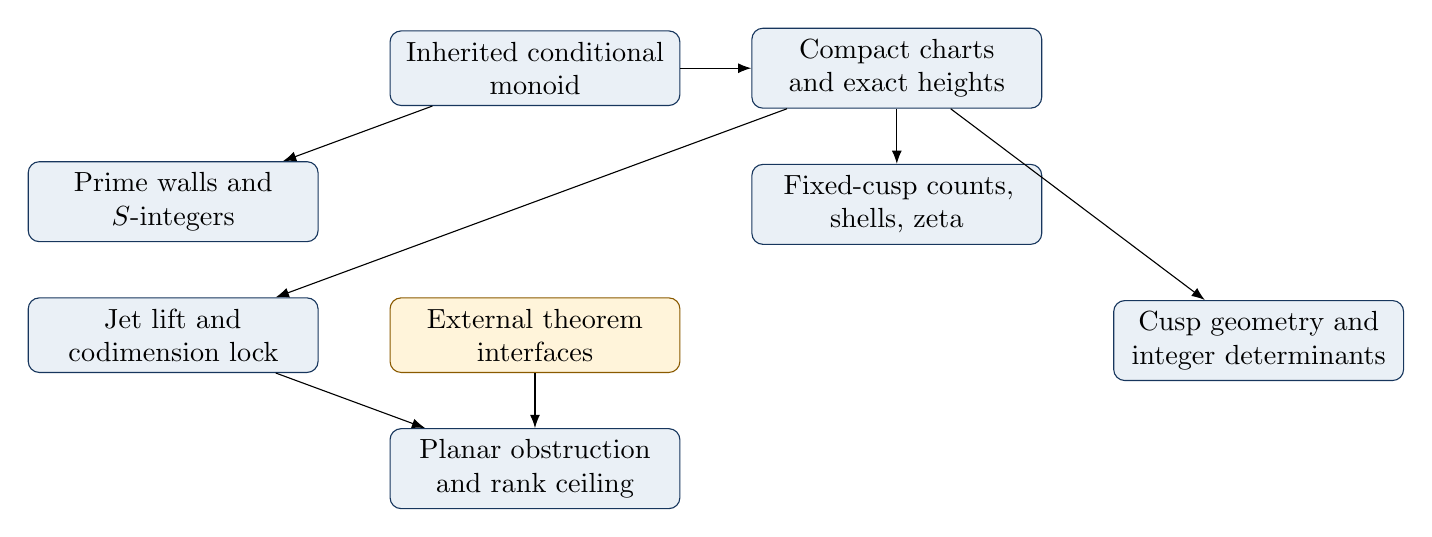
\begin{tikzpicture}[node distance=7mm and 9mm,>=Latex,
 n/.style={draw=navy,rounded corners,fill=bluegray,align=center,inner sep=4pt,text width=3.4cm},
 e/.style={draw=amber,rounded corners,fill=paleamber,align=center,inner sep=4pt,text width=3.4cm}]
\node[n] (old) {Inherited conditional\\monoid};
\node[n,right=of old] (charts) {Compact charts\\and exact heights};
\node[n,below=of charts] (counts) {Fixed-cusp counts,\\shells, zeta};
\node[n,below left=of old] (walls) {Prime walls and\\$S$-integers};
\node[n,below right=of counts] (geom) {Cusp geometry and\\integer determinants};
\node[n,below=of walls] (jet) {Jet lift and\\codimension lock};
\node[e,right=of jet] (ext) {External theorem\\interfaces};
\node[n,below=of ext] (obstruct) {Planar obstruction\\and rank ceiling};
\draw[->] (old)--(charts);
\draw[->] (charts)--(counts);
\draw[->] (old)--(walls);
\draw[->] (charts)--(geom);
\draw[->] (charts)--(jet);
\draw[->] (ext)--(obstruct);
\draw[->] (jet)--(obstruct);
\end{tikzpicture}
}
\end{center}


\section{Conclusions and present proof status}
\label{sec:conclusion}

\begin{summarybox}
The conjecture is not proved here.  The investigation nevertheless changes the shape of the target in five concrete ways.
\begin{enumerate}
\item It moves the problem to a \emph{fixed compact curve} without collapsing integer shifts.  Failure produces a quadratic, not linear, marked rational-point count.
\item It identifies exponent two as the exact unconditional ceiling for all rational points, by Six Exponentials, and separates the stronger rank-drop problem from the weaker one-sided \(S\)-integral problem actually needed.
\item It proves an exact prime-wall criterion in the possible rank-two group: harmless extra rational points must have foreign valuations of both signs; a counterexample is precisely a one-sided direction.
\item It proves two method obstructions.  Plain monomial determinants lose \(\asymp ND^{3/2}\) in a shell, and the natural differential approach is caught in a coefficient--codimension lock.
\item It exposes two high-leverage escape routes: cross-shell nonarchimedean divisibility for a scaling-covariant determinant, and a special codimension-two relation theorem for the diagonal three-dimensional lift.
\end{enumerate}
\end{summarybox}

The reciprocal compactification is the central new simplification.  It turns a counterexample into
\[
 \frac{T^2}{2\beta(\log3)^2}+O_\beta(T)
\]
unit-numerator rational points of logarithmic height at most \(T\) on the single compact cusp \(v=u^{\thetaq}\).  The logistic conjugate identifies the same set with coordinatewise Farey neighbors of the cusp \(1/1\).  These formulations preserve every conditional solution and remove the denominator-support qualification that burdened a generic all-rational criterion on the earlier normalized arc.

The full rational-point group is now completely bounded at the level available from classical transcendence: it is free abelian of rank at most two.  Rank one is the specialized Four Exponentials conclusion.  Rank two has quadratic all-rational growth, but it need not violate Alaoglu--Erd\H{o}s; the integral cone may be trapped on the natural ray by opposite foreign-prime walls.  This distinction suggests that an adelic sign theorem may be more attainable than full rational rank one.

The determinant analysis supplies a quantitative stop rule.  Total positivity makes every exponential alternant nonzero, and the unit-numerator condition makes the row-clearing lower bound exact.  Yet the optimal monomial shape still incurs
\[
 \delta_D\sim
 \frac{2^{3/2}}3\sqrt{\log2\log3}\,D^{3/2}.
\]
In a conditional shell with \(D\asymp N\) points, this becomes an \(N^{5/2}\) loss, larger than ordinary spacing gains.  The next determinant experiment should therefore measure common prime divisibility generated by orbit differences; any construction lacking a shell factor can be discarded without further optimization.

The 2026 algebraic-relation theorem is highly relevant but not directly applicable.  In dimension two, the transcendental slope forbids a nonzero polynomial vector field over a number field.  Promoting the slope or eliminating it by jets gives the same three-dimensional trajectory, where rationality fixes two coordinates and leaves a one-dimensional relation; the proven range requires dimension strictly below \(\sqrt3-1\).  Even a range extension must track its polynomial exponent below the exact shell threshold one.

No public source located during this work disclosed the rival team's claimed Alaoglu--Erd\H{o}s argument.  The report therefore cannot compare proof ideas.  It does provide a compact list of theorem-sized targets that a new claim can be tested against: Does it beat the quadratic fixed-cusp count?  Does it control the one-sided \(S\)-integral chamber?  Does it produce cross-shell divisibility of order \(ND^{3/2}\)?  Or does it break the dimension-three codimension-two lock?  A valid breakthrough should answer at least one of these questions with a rigorous new input.

\begin{targetbox}
The most concrete next calculation is the mixed Newton determinant from \cref{prob:semigroup-vandermonde}.  The most concrete next theorem is the diagonal-derivation special case \cref{prob:diagonal-special}.  They attack different sides of the same exact shell threshold and can be pursued independently.
\end{targetbox}

\appendix

\section{Nonduplication audit against the supplied unified report}
\label{app:nonduplication}
The supplied source is a very large unified document.  Before drafting this continuation, its section structure and key phrases were indexed.  The following table records the deliberate division of labor.

\begin{center}
\small
\begin{longtable}{p{0.31\textwidth}p{0.29\textwidth}p{0.31\textwidth}}
\toprule
Topic already developed in the supplied report & Treatment here & New replacement or refinement \\
\midrule
\endfirsthead
\toprule
Topic already developed in the supplied report & Treatment here & New replacement or refinement \\
\midrule
\endhead
Canonical least generator \(\beta\), unique semigroup coordinates & imported once as \cref{thm:inherited-monoid}; proof not repeated & used to obtain exact counts after a new injective compactification \\
Existing normalized compact arc modulo integer shifts & not rederived & reciprocal and logistic charts retain the shift coordinate and restore quadratic growth \\
Unbounded power-curve rational points and exponent-two heuristic & not repeated in its original form & fixed compact all-rational rank/count theorem via Six Exponentials \\
General valuation lattices and tropical/min-plus methods & not surveyed again & exact two-sign foreign-prime wall criterion in a rank-two basis \\
Generic determinant, Vandermonde, Pad\'e, and interpolation programs & no broad reprise & exact exponential-alternant nonvanishing and optimal \(D^{3/2}\) denominator-deficit theorem \\
Modulo-one/Sturmian shell coding & only the inherited count is used & fixed-cusp shell census, effective discrepancy, and height-zeta pole order \\
Analytic continuation, natural boundaries, special functions & omitted & discrete rational contraction dynamics and difference-\(D\) target \\
Earlier differential or Pfaffian observations & not duplicated & explicit planar number-field obstruction, two birational lifts, and exact codimension lock \\
Broad Lean inventory & not copied & module-level blueprint only for the new compactification, wall, jet, and deficit results \\
\bottomrule
\end{longtable}
\end{center}

Keyword checks in the supplied source found no prior occurrences of the defining logistic/unit-gap formulas, the reciprocal unit-numerator compactification, the 2026 relation-counting paper, or the coefficient--codimension terminology used here.  Some background themes necessarily overlap because they concern the same conjecture, but the theorem package and method audit are new deductions rather than rewritten sections.

\section{Elementary derivation of the conditional fixed-cusp count}
\label{app:lattice-count}
Assume failure and let
\[
 \Sol=\{n+k\beta:n,k\in\Nzero\}.
\]
Because \(\beta\notin\Q\), the parametrization is injective.  The number of solutions with \(t\le X\) is
\begin{align*}
 L_\beta(X)
 &=\sum_{0\le k\le X/\beta}
    \left(1+\left\lfloor X-k\beta\right\rfloor\right)\\
 &=\sum_{0\le k\le X/\beta}(X-k\beta)+O(X)\\
 &=\left(\frac X\beta+O(1)\right)X
   -\frac\beta2\left(\frac{X^2}{\beta^2}+O(X)\right)+O(X)\\
 &=\frac{X^2}{2\beta}+O_\beta(X).
\end{align*}
On the reciprocal chart, \(h(R(t))=t\log3\).  Substituting \(X=T/\log3\) gives
\[
 N^-_{\rm unit}(T)
 =\frac{T^2}{2\beta(\log3)^2}+O_\beta(T).
\]
For the logistic chart the exact height is \(\log(3^t+1)=t\log3+O(3^{-t})\); changing the threshold perturbs the count by \(O(T)\), so the same leading term holds.

For shell \([N,N+1)\), fix \(k\).  There is exactly one integer \(n\) with
\[
 N\le n+k\beta<N+1
\]
if and only if \(k\beta<N+1\); it is \(n=N-\lfloor k\beta\rfloor\).  Since \(k\beta=N+1\) cannot occur,
\[
 \#(\Sol\cap[N,N+1))
 =1+\left\lfloor\frac{N+1}{\beta}\right\rfloor.
\]

\section{Details of the lattice-weight asymptotic}
\label{app:deficit-details}
For completeness, the two elementary sums used in \cref{thm:deficit-asymptotic} can be obtained without a general lattice-point theorem.  Let
\[
 J_i(R):=\left\lfloor\frac{R-ai}{b}\right\rfloor
 \qquad(0\le i\le R/a).
\]
Then
\begin{align*}
 A(R)
 &=\sum_{0\le i\le R/a}(J_i(R)+1)\\
 &=\sum_{0\le i\le R/a}
   \left(\frac{R-ai}{b}+O(1)\right)\\
 &=\frac{R^2}{2ab}+O_{a,b}(R).
\end{align*}
Similarly,
\begin{align*}
 S(R)
 &=\sum_{0\le i\le R/a}
   \sum_{0\le j\le J_i(R)}(ai+bj)\\
 &=\sum_i\left((J_i+1)ai+\frac b2J_i(J_i+1)\right)\\
 &=\int_{\substack{x,y\ge0\\ax+by\le R}}(ax+by)\,dx\,dy
   +O_{a,b}(R^2)\\
 &=\frac{R^3}{3ab}+O_{a,b}(R^2).
\end{align*}
The error follows by comparing each unit lattice square with the Lipschitz integrand on the boundary triangle.  Inverting \(A(R)\) at the \(D\)-th weight and substituting in \(S(R)\) gives \eqref{eq:deficit-asymptotic}.

\section{A compact proof of the logistic derivative identities}
\label{app:logistic-calculus}
Write
\[
 L(z)=\frac{z}{1+z},
 \qquad
 F_{\thetaq}(X)=L\!\left(\left(\frac X{1-X}\right)^{\thetaq}\right).
\]
Since \(\logit F_{\thetaq}=\thetaq\logit X\), differentiation gives
\[
 \frac{F'}{F(1-F)}=\frac{\thetaq}{X(1-X)},
\]
which is the first derivative formula.  Taking a logarithmic derivative,
\[
 \frac{F''}{F'}
 =\frac{F'(1-2F)}{F(1-F)}
  -\frac{1-2X}{X(1-X)}.
\]
Substituting the first derivative yields
\[
 F''
 =\thetaq\frac{F(1-F)}{X^2(1-X)^2}
  \left(\thetaq(1-2F)-(1-2X)\right).
\]
For \(X>1/2\), put \(w=\logit X>0\).  The bracket becomes
\[
 -\thetaq\tanh(\thetaq w/2)+\tanh(w/2)<0,
\]
because \(\thetaq>1\) and \(\tanh\) is increasing.  Hence the graph is strictly concave on the marked half \((1/2,1)\).

\section{Glossary of the new objects}
\begin{description}[style=nextline,leftmargin=3.5cm]
\item[Reciprocal cusp \(\rec\)] The fixed compact graph \(v=u^{\thetaq}\) in \([0,1]^2\), parametrized by \((2^{-t},3^{-t})\).
\item[Unit-numerator point] A rational point \((1/m,1/n)\) with \(m,n\in\N\); exactly the image of an original solution.
\item[Logistic curve \(\logcurve\)] The rationally conjugate graph \(\logit Y=\thetaq\logit X\).
\item[Unit-gap point] A point \((m/(m+1),n/(n+1))\); each coordinate is Farey-adjacent to \(1/1\).
\item[Foreign valuation] A valuation of the first coordinate away from prime \(2\), or of the second away from prime \(3\), in a rank-two rational-group basis.
\item[Prime wall] A foreign valuation inequality forcing the second lattice coordinate \(k\) to have one sign.
\item[Monomial deficit \(\mathfrak d(\Lambda)\)] The gap between maximum row denominator weight and total column decay for an interpolation monomial set.
\item[Coefficient--codimension lock] The fact that dimension two permits the required point relations but not a number-field vector field, while legal lifts have dimension at least three and miss the proven relation range.
\item[Difference-\(D\) property] A proposed discrete analogue of the arithmetic \(D\)-property for rational contraction orbits at a nonanalytic cusp.
\end{description}

\begin{thebibliography}{99}

\bibitem{UnifiedReport2026}
\emph{The Alaoglu--Erd\H{o}s Integer-Exponent Conjecture: Unified Report},
supplied research manuscript, 22 August 2026.

\bibitem{AnthropicFable2026}
Anthropic,
``Claude Fable 5 and Claude Mythos 5,'' official announcement, 9 June 2026; redeployment update 1 July 2026,
\url{https://www.anthropic.com/news/claude-fable-5-mythos-5}.

\bibitem{Gao2026}
S. Gao,
``Counterexamples to the Jacobian conjecture in dimensions greater than two,''
\emph{arXiv:2608.00222}, 2026.

\bibitem{EpochHadamard2026}
Epoch AI,
``Hadamard Matrix of Order 668,'' FrontierMath Open Problems, 2026,
\url{https://epoch.ai/frontiermath/open-problems/hadamard}.

\bibitem{MathWorldRank2026}
E. W. Weisstein,
``Elliptic Curve Rank,'' \emph{MathWorld--A Wolfram Resource}, updated 23 August 2026,
\url{https://mathworld.wolfram.com/EllipticCurveRank.html}.

\bibitem{BHKKS2026}
G. Binyamini, N. Hirata-Kohno, M. Kawashima, and Y. Salant,
``Counting theorems for algebraic relations,''
\emph{arXiv:2604.15189v1}, version dated 11 August 2026.

\bibitem{Pila2007}
J. Pila,
``The density of rational points on a Pfaff curve,''
\emph{Annales de la Facult\'e des Sciences de Toulouse} \textbf{16} (2007), 635--645.

\bibitem{BNZ2024}
G. Binyamini, D. Novikov, and B. Zak,
``Wilkie's conjecture for Pfaffian structures,''
\emph{Annals of Mathematics} \textbf{199} (2024), 795--821.

\bibitem{Lang1966}
S. Lang,
\emph{Introduction to Transcendental Numbers},
Addison--Wesley, 1966.

\bibitem{BakerWustholz2007}
A. Baker and G. W\"ustholz,
\emph{Logarithmic Forms and Diophantine Geometry},
Cambridge University Press, 2007.

\bibitem{Karlin1968}
S. Karlin,
\emph{Total Positivity}, Vol. I,
Stanford University Press, 1968.

\bibitem{HCIZ}
Harish-Chandra,
``Differential operators on a semisimple Lie algebra,''
\emph{American Journal of Mathematics} \textbf{79} (1957), 87--120;
and C. Itzykson and J.-B. Zuber,
``The planar approximation. II,''
\emph{Journal of Mathematical Physics} \textbf{21} (1980), 411--421.

\bibitem{KuipersNiederreiter}
L. Kuipers and H. Niederreiter,
\emph{Uniform Distribution of Sequences},
Wiley, 1974.

\end{thebibliography}

\end{document}
